\documentclass{book}
\usepackage[utf8]{inputenc}
\title{paper presentation Template}
\date{5th April  2019}
\usepackage{amsmath}
\usepackage{graphicx}
\graphicspath{{./img/}}

\usepackage{fixltx2e}
\usepackage{todonotes}
\usepackage[utf8]{inputenc}
\usepackage{svg}
\usepackage{newunicodechar}
\newunicodechar{fi}{f}
\usepackage{hyperref}
\usepackage{tabularx}
\usepackage[left=2cm, right=5cm, top=2cm]{geometry}
\usepackage{lscape}
\usepackage{multirow}
\usepackage[shortlabels]{enumitem}
\usepackage{cleveref}
\title{}
\author{}

\newcommand{\jk}[1]{\todo[inline]{JK: #1}}
\begin{document}
\title{\Large Integration of Autonomous and Human-Driven Cars     \\ Review Meeting}




\begin{titlepage}

\newcommand{\HRule}{\rule{\linewidth}{0.5mm}}

\center

%----------------------------------------------------------------------------------------
%	TITLE SECTIONS
%----------------------------------------------------------------------------------------

\HRule \\[0.4cm]
{ \huge \bfseries Integration of Autonomous and Human-Driven Cars}\\[0.4cm]
\HRule \\[1.5cm]

%----------------------------------------------------------------------------------------
%	AUTHOR SECTION
%----------------------------------------------------------------------------------------
\begin{minipage}{0.4\textwidth}
\begin{flushleft} \large
\emph{Author:}\\
Ekene Frank \textsc{Ozioko}
\end{flushleft}
\end{minipage}
~
\begin{minipage}{0.4\textwidth}
\begin{flushright} \large
\emph{Supervisor:} \\
Dr. Julian \textsc{Kunkel}
\end{flushright}
\end{minipage}\\[1cm]
~
\begin{minipage}{0.4\textwidth}
\begin{flushright} \large
\emph{2nd Supervisor:} \\
Dr. Frederic \textsc{Stahl}
\end{flushright}
\end{minipage}\\[1cm]

%----------------------------------------------------------------------------------------
%	 DETAILS SECTION
%----------------------------------------------------------------------------------------
\setcounter{tocdepth}{1}
\textbf{\LARGE PhD Confirmation Report }\\[2.8cm]
\text{\Large Department of Computer Science }\\[1cm]
\text{\Large School of Mathematical, Physical, and Computational Sciences }\\[1cm]
%----------------------------------------------------------------------------------------
%	LOGO SECTION
%----------------------------------------------------------------------------------------

\includegraphics[width=0.15\textwidth]{logo}\\[1.5cm]
\textsc{\large University of Reading }\\[1cm]

%----------------------------------------------------------------------------------------
%	DATE SECTION
%----------------------------------------------------------------------------------------

{\large \today}\\[2cm]


%----------------------------------------------------------------------------------------

\vfill % Fill the rest of the page with whitespace

\end{titlepage}
\chapter*{Abstract}
%\begin{abstract}
	Here is where I would say what is in this document(Abstract).
%\end{abstract}

\tableofcontents
\newpage

%\section{Section}

%Dummy text

%\subsection{Subsection}



\chapter{Introduction}

\label{Introduction}
Over the years, gridlock and accidents at road traffic intersections  has been increasing progressively due to increase in the number of cars without the right compliment of road infrastructure and traffic management techniques. Drivers are sometimes forced to wait through several minutes or hours before accessing the intersection facility. Gridlock at intersection  \Cref{fig:intersectioncrash} without good traffic management strategies leads to ripple effect: frustration incidence of road rage, traffic backup in other intersections, forces pedestrians out of the crosswalks, to mention but a few.
The current research direction on traffic management mostly focuses on the situation where all vehicles are fully autonomous. However conventional vehicles are human-driven and will need to transition through regimes featuring a varying proportion of human-driven and autonomous vehicles ratio before realizing such a fully autonomous based future in accordance with \cite{kuramoto2018mono, seshia2016towards}. Based on the foregoing, we need to address the safety issues in a hybrid system for the coexistence of human and autonomous vehicles as represented in fig \ref{fig:Crossjunction}. The update from  incidents involving autonomous vehicles has already highlighted the need to research directed towards the safety of autonomous vehicles co-existing with human-driven vehicles\cite{le2015autonomous, wang2015longitudinal,liu2018safe, lu2004automated, ma2017parsimonious, zhao2019bilevel, lin2019autonomous, rios2017survey, van2001prototype, huang2017safety}.
The transition to the autonomous driving system has generated various expectations ranging from the decrease in traffic accidents/incidence, decrease in traffic congestion, increase in roads comfort, decrease in carbon emission, decrease in fuel consumption  and to a shortage of drivers. Within this envisaged transition period of coexistence of human-driven and autonomous vehicles, there is a need for a robust technology to be put in place to drive the process. Under these conditions, it will not be too feasible for the human car drivers to predict the movements of an autonomous car and vice versa. However, there has been an established worry over the road traffic control system due to constant traffic congestion caused by increased population and urbanization.\\
\begin{figure}
\centering
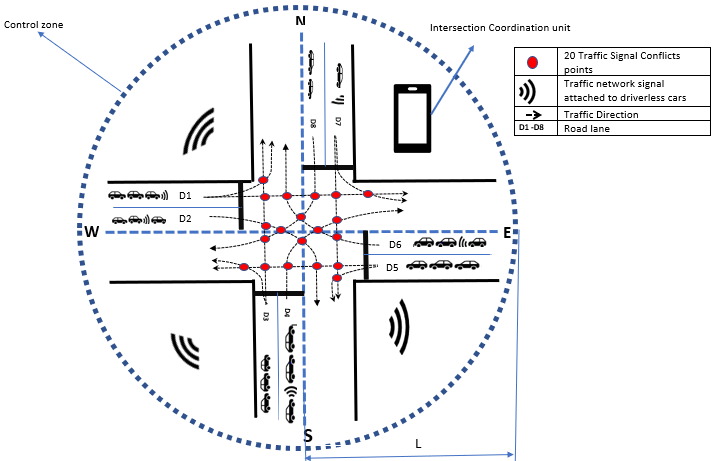
\includegraphics[width=15cm,height=10cm]{crossjunction1}
\caption{Crossroad intersection with double lanes}
\label{fig:Crossjunction}
\end{figure}



\begin{figure}
%\centering
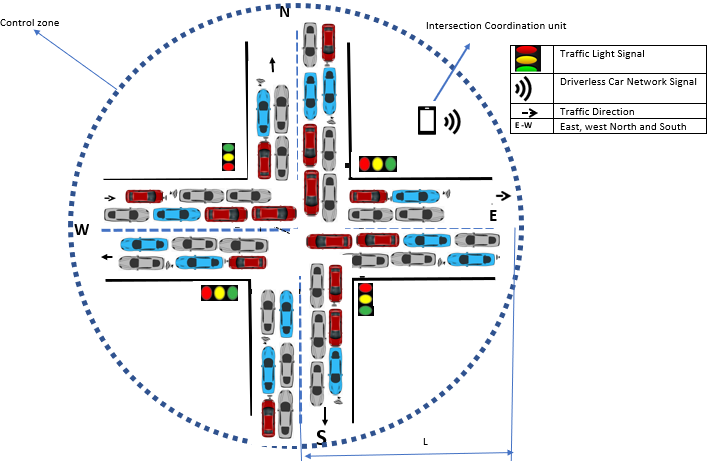
\includegraphics[width=12cm,height=10cm]{intersectioncrash}
\caption{Traffic Jam at Cross intersection}
\label{fig:intersectioncrash}
\end{figure}

\begin{figure}
%\centering
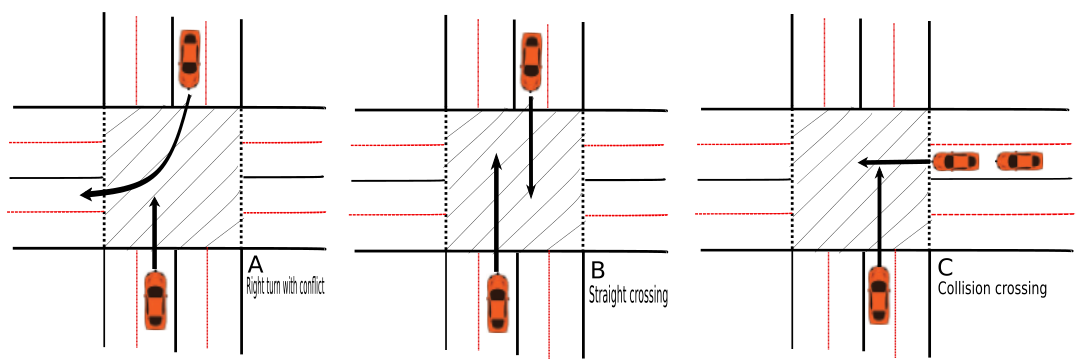
\includegraphics[width=14cm,height=4cm]{diffcrossingscinerios.PNG}
\caption{Different scenarios of intersection crossing (A,B,C}
\label{figIntersection scenerios}
\end{figure}

\textit{\color{red}} As this document is work in progress and developed alongside the project.
For the convenience of the reviewers, the current status of the research is outlined in \Cref{sec:researchstatus}. Road traffic intersection point is a region shared by two or more roads. This intersection region is assigned for sharing by vehicles from different road lanes and directions to reach their destination or goals. The fundamental work of intersection is to path direction for vehicles. Traffic intersection are of different categories depending on the number of roads system accessing it  and they are complex areas of the road system. Vehicles moving in several direction access same space at the same time. In this case, drivers must make part moment choice at an intersection point by considering his route, crossing point geometry, speed and heading of other vehicles etc. A little mistake at road intersection points in judgment or decision points on path trajectories can cause serious accidents. It causes delay and it depends on type, geometry, and type of control. By and large activity stream depends on the execution of the convergences road system. It also affects the capacity of the road. Therefore, both from the accident perspective and the capacity perspective, the study of intersections is very important for the traffic engineers especially in the case of
urban scenario. An early approach to automation in the field of vehicles started with the Automated Highway System (AHS) research program\cite{horowitz2000control}, it focused on the improvement of the capacity and the safety of highway traffic. The efficient scheduling of the traffic lights system at road intersection can only guarantee an optimal utility of the road infrastructure at the point of intersection\cite{schrank2012tti}. The advent of automated vehicles led to the birth of vehicle-to-vehicle and vehicle-to-infrastructure communication which inadvertently led to road intersection settings without traffic lights but has smooth and efficient flows of traffic with good safety measures. There is no doubt in saying that connected and automated vehicles (CAVs) have the potential to improve safety by reducing and mitigating traffic accident with seamless flow of traffic and good safety measures.  In the traditional traffic control paradigm, traffic flows at intersections are regulated by traffic lights or signs that restrict the maximum traffic handling capacity of the intersections and increase inconveniences of frequent stops and idle time. Vehicles at a stop sign must come to a complete stop before crossing, even if no other vehicle is present at the road segment thereby causing traffic delay. In a similar way but without any traffic sign, traffic entering the roundabout must yield to traffic already in the circle. At busy intersections, flows of vehicles on each approach are usually regulated by green and red lights that eventually increase the stop delays.	 Among the various methods of alleviating traffic congestion, traffic-light or signal control is commonly considered as the most effective method, and various strategies for urban traffic management have been developed based on this approach\cite{papageorgiou2003review,treiber2000congested,kamal2012control}. Their signal control strategies can only partially improve the traffic flow if all approaches to the intersection are not equally congested, and they cannot eliminate the stop delay of vehicles at intersections regardless of traffic volume. Considering increasing trends of vehicles and sustainability of the road transportation system, a breakthrough in the intersection control paradigm which may eliminate the necessity of stops and increase the capacity of intersections, is highly expected.\\
The advancement in sensor technology and adoption of communication technology is increasing the penetration rate of driver-less vehicles. The advantages of the high-precision abilities which autonomous vehicles have over human driven vehicles are of great important to feature research in autonomous intersection scheduling scheme.	The scheme efficiently utilizes the intersection area by preventing each pair of conflicting vehicles from approaching their cross-collision point (CCP) at the same time instance, instead of reserving the whole intersection area for the conflicting vehicles successively. Moreover, the introduction of relevant constraints ensures the scheme is free from any collisions and enables it to manage turning movements of the vehicles under a safe velocity limit. Turing vehicles sometimes need special treatment so that multiple vehicles can slowly and closely cross the intersection, which is realized in our model. An intersection coordination unit (ICU), which is installed at the intersection, uses two-way communication to receive basic driving information from the approaching vehicles, for instance: current position, velocity, and destination at the next intersection and sends real time guidance to them after computing their control inputs. 	In the scheme, a risk function is proposed that explicitly indicates only a portion of the intersection by quantifying the risk of a collision of a pair of vehicles around their CCP. More specifically, at any time, if two conflicting vehicles are very close to their CCP, the risk function returns a high value, and if at least one vehicle is far from the CCP, the risk value returns a negligible value. Considering states of all vehicles, a constrained nonlinear optimization problem is solved in a model predictive control (MPC) framework in order to let the vehicles cross the intersection rapidly by minimizing the total quantified risks of all vehicle pairs. Minimization of risks helps in generating safe trajectories of vehicles by reducing unused time and space in the intersection area and consequently, enhances the traffic handling capacity of the intersection and improves traffic flows. However, the scheme integrates fully automated vehicles intersection to improve traffic operations. The proposed model will be evaluated through numerical simulation and its performance is compared with the traditional signalized and mixed traffic scheme. Under the various traffic-flow conditions, the key interest to observe is the stop delay of vehicles at intersections is almost eliminated and flows of vehicles and the capacity of the intersection are significantly improved.  The semi-automated and the fully automated vehicles are controlled by the sensor technology with  communication languages. The communication must happen between vehicle to vehicle or vehicle to infrastructure seamlessly. Human driven and autonomous vehicle intersection scheme with light and light-less under a connected vehicles environment that overcomes the limitations of the existing methods is proposed.\\
The novelty of the proposed scheme is the global coordination of vehicles at the intersection area, by considering the states of all vehicles at real time basically on avoiding their meeting at their cross-collision points. However, considering the increasing trends of vehicles and sustainability of the road transportation system, a breakthrough in the intersection control methods, which may eliminate the necessity of stop and increase the capacity of intersection, is highly expected. Conventional drivers create traffic congestion due to the various types of disturbances ranging from the state of mind of the driver to roadside distractions, therefore, people on daily bases waste a considerable amount of fuel and time, and that is why the cost of traffic increases day by day. Exceeding the number of vehicles meant for a road system capacity is the main reason for traffic congestion as the density of traffic is higher than the road network capacity in most cases. In this situation, if the existing road system is used in a very innovative and efficient way, then this problem situation can be solved. Management of intersection and various controlling strategies for a mix traffic are feasible solution to a mix vehicle situation.\\
However, to control traffics at intersections without traffic light, various mathematical parameters are involved which are related to the interface of the vehicles being control. Geometry is one of the important tools which is used here to control the traffic without the light signals. These parameters are classified according to the movement's dynamics the vehicles. There is a  potential cause of harm in safety-critical situations for artificial intelligent system  such as autonomous driving cars which has been gaining research attention in recent time.
For instance, decision making at intersections in autonomous vehicles is either solely based on machine learning, through end-to-end intersection control unit, or involves some combination of logic-based reasoning and machine learning components, where an image classifier produces a classification, say speed limit or a stop sign, that serves as input to a controller \cite{huang2017safety,amodei2016concrete,seshia2016towards}. A system that was able to detect that presence of another vehicle approaching a cross was developed \cite{milanes2010controller,claes2011decentralized,zeng2015novel,eguchi2007discrimination}. Lane detection scheme is very important in road transportation system especially as it regards autonomous vehicle for essential lateral services such as lane departure warning system and lane keeping assistance system. Furthermore, detected lane could be considered as an indication to vehicle's further driving path as it could be a principal criterion to decide how forward obstacle could be affected or not. In another word, lane detection could not only affect longitudinal systems such as autonomous emergency braking system, forward collision warning system, and adaptive cruise control system but also indirectly affect full spectrum of the automated driving system\cite{song2017novel,dickmanns1992recursive,kim2008robust,siogkas2013random}. Risk factors associated with autonomous vehicle sensor failures can be mitigated by using the method of single failure assumption which states that at most one sensor can fail at any time, however, the detection of the failures in autonomous vehicle sensors  systems is generally carried out by simple algorithms which can improved our objective to developed a model-based fault-tolerant control-scheme for vehicle lateral dynamic control. This approach can detect and identify sensors failures right after failure has taken place. "Then the output of the faulty sensor is reconstructed from the output of the healthy ones \cite{oudghiri2007fuzzy,kienke2000automotive,staroswiecki2005fault} This process is called "Sensor data reconstruction using bidirectional recurrent neural network". Furthermore, it is intended  that as the number of autonomous vehicles on the road increases, traffic delays decrease monotonically based on the level of intelligence and rapid response to control or instruction work.



\section{Motivation}
\label{sec:motivation}
Driver-less cars are emerging while the conventional or human driven cars cannot be automatically phased-out from the road, hence the need for a mix traffic scenario on road system at the point of intersection. While recent surveys reveal fear of driving or riding in self-driving vehicles is on the rise, a new study predicts that the global autonomous vehicle market will grow more than tenfold from 2019 to 2026 \cite{yun2016relationship}.
The study from Portland, Ore.-based "Allied Market Research"  concludes  the global market for autonomous vehicles will be worth \$54.23 billion in 2019 and increase to \$556.67 billion by 2026 with a compound annual growth rate of 39.47\% during that period \cite{krasniqi2016use, williams2019reliance}. Rise in the development of smart cities is expected to significantly drive the Autonomous Vehicle penetration. CO2 emission and the growing numbers of cars on the road raises an issue of concern in relation to environmental pollution and traffic management. The major motivation for this research can easily be summarized as shown below
\begin{enumerate}
   \item Cost of autonomous vehicles (AVs) is higher and not affordable by everyone. The systems of AVs are high because it uses namely sensors, radar, and communication devices high insurance, or maintenance costs, which are costly compared to older (less safe) vehicles which uses cheap and affordable devices. This raises questions about the affordability of life-saving technology for those (the masses) who need it most \cite{wadud2017fully, childress2015using}.
   \item Full enabling environment for AVS are not in place yet. Currently millions of pounds are being invested on research in smart roads system, defining and creating technologies, frameworks and standards \cite{fagnant2015preparing}, to ensure safe operation, and that exactly the right data flows between vehicles and the environment around them. The development of a city usually starts with a city master plan, but as new not envisaged technology comes up, altering the master plan is usually a herculean task because of cost, and litigation's is followed. In most cases it will cost more to reconstruct an existing facility than to build a new one because of a lot of constrain ting factors \cite{legacy2019planning, bahamonde2018systemic}
   \item Need for redesign or Constructing new roads for AVs: In order to stay on the road, avoid collisions and obey traffic laws, AVs rely on a series of sensors that help the cars understand the environment in which they're traveling in real time. By using a combination of ultrasonic, radar, imaging processing and sensors, a digital road map is formed ahead of an AV to essentially help it "see" where it's going \cite{dickmann2016automotive, essati2016method}. This has a grave impact on the current road system coupled with the cost of implementation
   \end{enumerate}

However, it is a general knowledge and an established worry over road traffic control system due to constant traffic congestion caused by increased population and urbanization.  It has become hard for traffic  controllers to provide safe and efficient traffic movement on the road at the same time. The connections of different road paths make intersections, where the possibilities of vehicle collision are critical without good control measures. Traffic congestion often occurs when traffic density becomes higher than the capacity of a road or road network. Efficient use of the existing road infrastructure by innovative intersection management and control is a solution for the cities where further construction and expansion of roads are difficult. Conventional vehicles have   road traffic intersection control measures of using traffic light system, while the driver-less vehicles came in with new technology for accessing the road facilities involving vehicle-to-vehicle and vehicle-to-infrastructure communication, while human driven vehicles involve driver-to-road infrastructures communication. Considering the fact that the introduction of new technology is not automatic and the current technology will be replaced by new one gradually, hence the need for the integration of driver-less vehicle movement parameters with that of human driven vehicle to midwife the smooth transition to a fully automated road system. This is necessary because conventional vehicles which are currently occupying the road cannot just be phased out sooner based on the following constraints: cost, choice, infrastructure, etc. Realistic point of view has it that a new technology which will phase out the existing ones will normally take some time for the integration and acceptance because in most human driven vehicles users believes in the way they used to do it and cannot afford to do away with their private vehicle immediately even with some government incentives if available. Gradual transformation to a fully automated road transport system can seamlessly be achieved by integrating the attributes of automated vehicles into the human driven vehicles bearing in mind the human driver’s attribute on road (tracking user's stochastic behaviour) and communication parameters. Among all the human driven vehicles traffic controlling methods, the traffic light signalling method is the most effective and secure, but this traditional method increases the amount of delay time due to stops and lane schedule, then for this reason, various automated vehicles and semi-automated vehicles will be faced with various delay problems \cite{wen2019solving}\\ .

\section{Research Progress}
The following progress was made on the course of this research:

\begin{enumerate}[(a)]
    \item Clarification of the research goal: We define research strategies and implementation steps starting with the development of a physical model of traffic simulator
    \item Definition of a methodological research approach: Preliminary experimental research was conducted with a randomly moving vehicle  that forms a baseline for our research.
    \item Background research: We developed a 10-page document summarizing the traffic intersection management techniques with their pros and cons
    \item Model creation: a car motion model was developed based on physics principles.
    \item Simulator prototype: A Python3 prototype has been developed. Is uses the \textit{continuous simulation} approach approximated with discrete time steps.
    While still premature, it showcases how to build an environment of intersections, uses a simplified model, and provides debugging output to understand the behaviour of cars using Scalable Vector Graphics (SVG) reporters combined with other functions.
\end{enumerate}

%\jk{Integrate the stuff here}
 % Python and there have been a regular weekly meeting from 3rd December 2018 to date which has been very helpful %towards an in-depth understanding of the subject area, motivated  and was focus on my research. Based on the state %of the art in traffic management, I have done a background research, developed a matrix of the methods used, %proposed my method and have started developing the physical model.


%\paragraph{Other activities}

%At the beginning of April, I gave my first presentation about my research as part of the Open Source AI workshop\footnote{\url{https://ossg.bcs.org/blog/event/open-source-ai-april-2019/}}.
%Preparing and giving a technical presentation about my research was a rewarding experience.

\section{Research Question}
\label{sec:question}
\begin{itemize}
\item Can a vehicle  mix coexist in a road traffic intersection area ( mix of human-driven and driver-less cars)?
%\item Can the behaviour of a human driver and that of an autonomous car be integrated into one system?
\item What impacts will autonomous cars have on the human-driven cars upon integration?
\item What strategies can be used to deal with the mix traffic scenario for an efficient and safe intersection management?
\end{itemize}

\section{Contribution to Knowledge}
\label{sec:contribuion}
This thesis describes the use of appropriate modelling and optimization techniques to investigate the different traffic control strategies which can be applied to a mix traffic setting combining both traffic lights and light-less vehicles and drivers communications at intersection

However, the main areas of our contributions are as follows:
 \begin{itemize}
 \item Development of a mix traffic intersection model.
 \item Validation of an alternative strategy for conflict resolution at cross collision point in an intersection area
 \item Comprehensive survey and critical discussion of the state-of-the-art in traffic management with a development of a classification matrix for different strategies of intersection management.
 \item Identification of the challenges and obstacles for the co-existence of autonomous and human-driven cars in a mix traffic setting
\item Design of a tool architecture for development of scheduling and optimization algorithms in the Python environment
\end{itemize}

\section{Research Objective}
\label{sec:objective}
The objectives of this research were set as follows:
\begin{itemize}
\item Review the different traffic control strategies for managing traffic  intersection and propose an alternative strategy for controlling human-driven and driver-less vehicles in an intersection setting.
\item Modelling and simulation of an efficient and save traffic intersection management for a mix vehicle environment.
\item Based on physical driving models and the psychology of human drivers, evaluate performance of various scenarios of the vehicle mixes and compare to the alternatives
\end{itemize}


\section{Research goals}
\label{sec:goals}
Our research main goals are summarized as follows:

\begin{itemize}
\item To develop a simulator model for a road traffic junction and use it to investigate strategies for safety and improvement in traffic flow in a vehicle mix environment
\item Develop the model based on the behaviour of human drivers and that of driver-less cars.
\item Investigate the performance of the method based on the percentage mix of HVs and AVs to serve as a guide for the transition period.
\end{itemize}

This high-level goal can be organized into the following sub-goals:
\begin{enumerate}
    \item Review of existing traffic management strategies, and proffer a robust and efficient traffic intersection management for a mix traffic
\end{enumerate}

However, this thesis focuses on modelling and optimization of a mix traffic intersection techniques to improve efficiency of light-controlled intersections in combination with vehicle-to -vehicle and vehicle-to-infrastructure communications. In addition, the objective of this work also involves the review  of the different traffic control strategies that’s is applicable to a mix  traffic setting which will reduce traffic congestion , increase road safety measures and drive the transition to fully autonomous intersection system.



\section{Research Methodology}
\label{sec:methodology}
The	need	for	 a mix traffic is	identified	and	various	options	for	addressing this	need	are	considered	and	analysed.	We considered intersection	key	terms	and	discussed the intersection	users,	configurations,	traffic	control,	capacity,	and	quality	of	service.
In addition, the	ranges	of	physical	dimensions	and	the	operational	characteristics	of	each	intersection	design	element were considered.


\begin{figure}
\centering
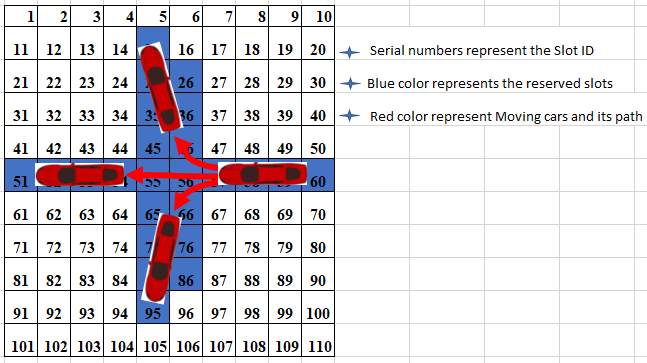
\includegraphics[width=8.5cm]{tiles}
\label{considerations}
\caption{Reservation slot}
\label{fig:tilesslot}
\end{figure}

\begin{figure}
\centering
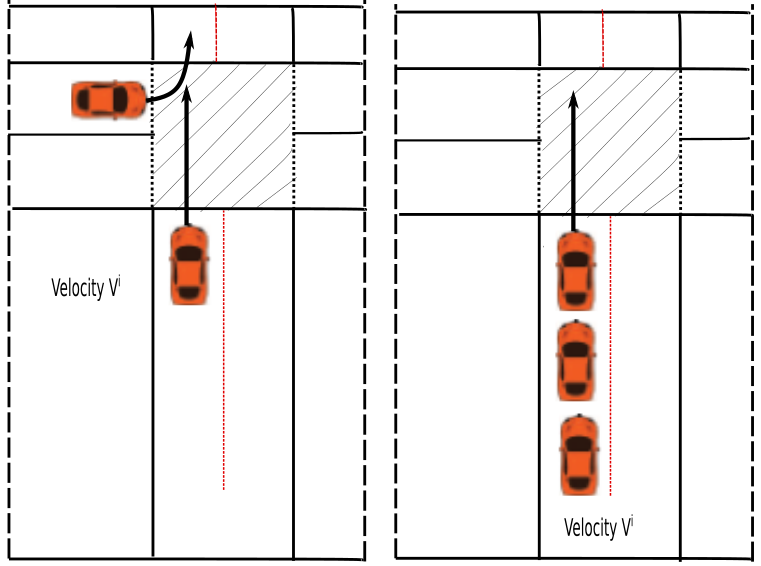
\includegraphics[width=6.5cm]{conflicscenerio}
\caption{intersection Conflict}
\label{fig:intersectionConflict}
\end{figure}

\begin{figure}
\centering
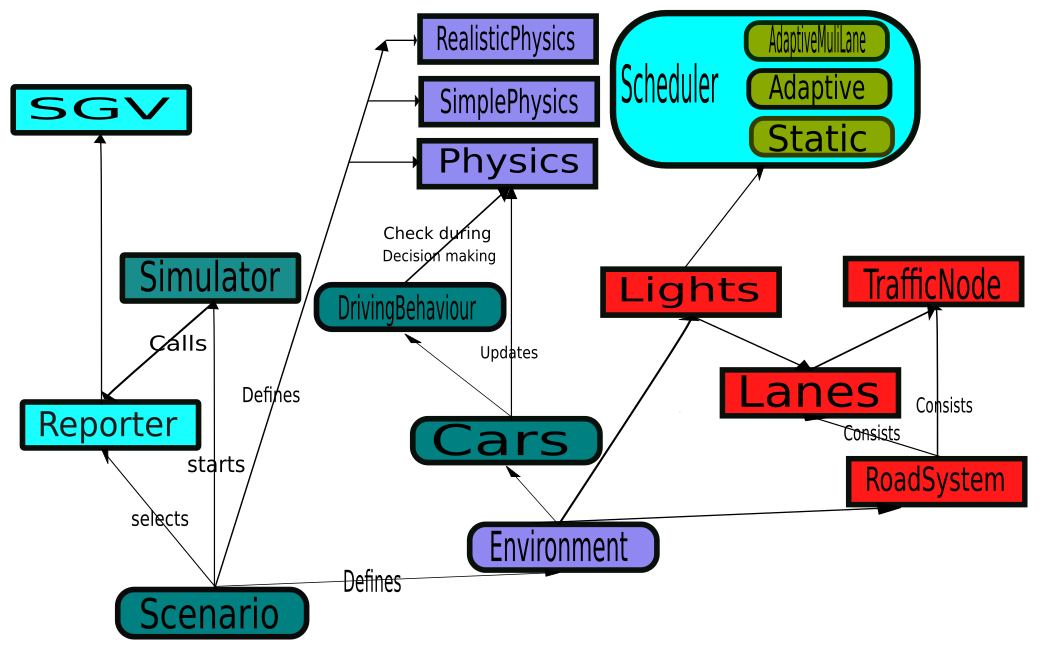
\includegraphics[width=15cm]{Componentsodg}
\caption{Components Diagram}
\label{fig:componentsdiagram}
\end{figure}

\section{Scope of Research}
\label{scope}
In the course of this project, we considered two main types of traffic intersections:
\begin{itemize}
    \item T-intersection: This involves a three road system intersecting at a point
    \item +-intersection:  This involves a four road system intersecting at a point
The above two categories of intersection have some other properties like single lane where cars move only in one direction, dual lane system.
This was robustly tested with both good and wrong data
\end{itemize}



\section{Organization of the Thesis}
\label{sec:organization}
This thesis is organized as follows: Chapter 1 covers the introduction, motivation, research objectives and questions, goals, methodology, consideration, scope and contribution to knowledge,  with the review of related works in chapter 2. Chapter 3 presents a dynamic traffic model which can adopted to different intersection scenarios. Revolving around these mentioned challenges in \cref{sec:motivation}, the goals for the thesis are listed in \Cref{sec:goals} which has the  potentials to address the above-mentioned challenges. The relevant research questions are derived in \Cref{sec:question} while the key contributions of this work in relation to the state of the art are enumerated in \Cref{sec:contribuion}. Then, the research methodology is described in \Cref{sec:methodology}.

\section{Status of the Research}
\label{sec:researchstatus}
A traffic model have been developed, we are now using it to review different strategies for managing traffic within different scenarios and different traffic intersection types: The current results obtained from the implemented experiments are as attached.

\section{Conclusion}
While reflecting on my experience in the course of doing this research, I came to realize that research in the area of mix traffic though very challenging but interesting once one starts producing results which reflect the expected model outputs. The experimental process needs resilience and persistence but is enjoyable at least in the subject area. However, I am passionate about learning things that concern to my major and future career to be able to contribute a novelty in the sector. This informs why I came into this process optimistic of finding to find something new. Though I originally have an idea in traffic management, after spending some time researching about the current state of the art, I can now say I have something new to add which is futuristic.


\chapter{Related Works}

\section{Introduction}
This chapter covers a detailed review of the different traffic management strategies with its pros and cons. In addition, it contains a matrix of categorization of the traffic management scheme with comparison to other methods.  Traffic management systems are composed of a set of application and management tools to improve the overall traffic efficiency and safety of the road  transportation systems. This has been in the eye of research for decades because of increasing population and urbanization. There has being a lot of improvement in traffic management strategies over the years.\\

 It has become hard for traffic  controllers to provide safe and efficient traffic movement on the road system at the same time. The interconnections of different road paths make intersections, where the decision and possibilities of vehicle collision are critical without good traffic control measures \cite{ferreira2015methods,feng2015real}. The Efficient use of the existing road infrastructure by innovative intersection management and control is a feasible solution for the cities where further construction and expansion of roads are difficult. Conventional vehicles have   road traffic intersection control techniques of using traffic light system, while the driver-less vehicles access road facilities via communication platforms: vehicle-vehicle and vehicle-infrastructure communication. The human-driven vehicles only involve driver-to-road infrastructures communication (one-way communication). The deployment of new technology is not usually automatic, and the current technology will be replaced by new once gradually, the integration of driver-less vehicle movement parameters with that of the human-driven vehicle to midwife the smooth transition to a fully automated or smart city is necessary.\\
An early approach to automation in vehicles started with the Automated Highway System (AHS) \cite{horowitz2000control, horowitz2000control,lu2004automated, vial2016scheduling, annell2016probabilistic}, it focused on the improvement of the capacity and the safety of the highway road traffic system. The advent of automated vehicles led to the birth of vehicle-to-vehicle and vehicle-to-infrastructure communication which inadvertently led to road intersection settings without traffic lights but has smooth and efficient flows of traffic with good safety measures. There is no doubt in saying that connected and automated vehicles (CAVs) have the potential to improve safety by reducing and mitigating traffic accident with seamless flow of traffic and good safety measures \cite{schrank2012tti, rios2017survey, lin2019autonomous, abduljabbar2019applications}.\\

%\section{Why is this interesting/useful}
%Gradual transformation to a fully automated road transport system can seamlessly be achieved by integrating the %attributes of automated vehicles into the human driven vehicles bearing in mind the human driver’s attribute on %road (tracking user's behaviour) which is stochastic in nature. Among all the controlling methods of traffic %de-congestion, the traffic light signalling method is the most effective and secure, but this traditional method %increases the amount of delay time, and for that reason, various automated vehicles and semi-automated vehicles %will be faced with various delay problems

%\section{Review of Related Literature's}

%Currently, various studies which are being conducted in the area of traffic intersection control assumes a traffic environment of autonomous vehicles mainly, Lee et al\cite{lee2012development} proposed an algorithm where vehicles request a travelling course to avoid collision but it assumes all vehicles are AV . There are some studies for the fully mixed environments, \cite{hara2018vehicle} but focus was on straight roads, which investigated and quantified driver behavior changes due to the spread of autonomous vehicles \cite{hara2018vehicle} . We focus on  a hybrid intersection with platooning, and clarify how to cope with traffic flow such that it does not require braking under mixed environment. Omae et al \cite{omae2010automatic} Proposed reducing the time it takes for a vehicle to pass through an intersection using VIVC (Vehicle to Vehicle communication) and IVC (Infrastructure to Vehicle communication) technology. However, their experiments assumed that the vehicles passing through the intersection were autonomous vehicles implementing ITS (intelligent transportation system) functions, and the mixed environment was not taken into consideration. Guni Sharon et al.\cite{kamal2015vehicle} also proposed an intersection entry using a traffic signal that has sensing technology to detect non-autonomous vehicles, as well as technology that communicates with autonomous vehicles. Though this study showed positive results, the implementation of this traffic management system is dependent upon the existing infrastructure, and the technology is potentially cost ineffective\\


\section{Classification Matrix for Traffic Intersection Management Techniques} Based on the current state of the art in vehicle technology and road traffic management system as it relates to human-driven and driver-less vehicles, we have two main methods of controlling traffic flow within an intersection, this includes:\\

\begin{itemize}
    \item \textbf{Traffic signal light}: This consists of the installation of signal lights that control traffic streams by using different light indicators. Its primary aim is to prevent simultaneous movement of two or more incompatible traffic schedule of phases by assigning and cancelling the right-of-way to a set of traffic schedules \cite{omae2010automatic, van2006impact, kamal2012control, treiber2000congested, papageorgiou2003review}.

 \item \textbf{V2V and V2I Communication}: This involves a traffic intersection control schedule without lights, in this case, autonomous or semi-autonomous vehicle accesses an intersection using vehicle to vehicle (V2V) or  vehicle-to-infrastructure (V2I) communication means \cite{ kamal2015vehicle, fajardo2011automated, au2015autonomous, montanaro2018towards, uno1999merging}.
\end{itemize}

However, we categorize the above two methods of implementing a traffic schedule into two distinct strategies  based on the two-underpinning factor:  centralized and decentralized strategies.

\subsection{Centralized approach}: In the centralized method as reflected in table 1, there is at least one factor in the traffic scheduling characteristics or features that are globally decided for all vehicles in the scheme by a single central controller. When a central decision is made for at least one of the factors, it is called a centralized approach \cite{milanes2010controller, litman2017autonomous, anderson2014autonomous, seshia2016towards}.

\subsection{Decentralized approach}: In this category, all the vehicles are treated as autonomous agents but use the interaction between  (vehicle-to-vehicle and vehicle-to-infrastructure) to maximize efficiency in communication and control. In this case however, each individual agent (vehicle) obtains information from other vehicles and or road-side infrastructure to enhance performance criteria like safety, efficiency and travel time before access sing the intersection \cite{claes2011decentralized,dresner2008multiagent, zeng2015novel, eguchi2007discrimination, ferreira2015methods, knorn2014passivity}.\\
The correlation used in intersection control with the underpinning technologies with the evaluation of its performance matrix is as shown in table 2. Each matrix cell defines the performance index of various methods and identifies which characteristics are to balance. This matrix presents a detailed picture for consideration in the development of a robust hybrid-based system with some degree of safety, performance, costing and adaptability.

The classification categories are based on the below column headers:

\begin{itemize}
	\item \textbf{Method}: the control  or strategy to orchestrate the traffic flow, i.e., the rules deciding which car may drive or must wait?

	\item \textbf{Vehicle Type}: For autonomous vehicle (AV) and or human-driven vehicle (HV): the type of vehicle it  is controlling: Hv is a human-driven vehicle while Av refers to autonomous vehicles
	\item \textbf{Performance index}: This is a measure of intersection efficiency: where +, ++ means good and best performance respectively.
	\item \textbf{Communication means} Signal, vehicle to vehicle (V2V) or vehicle to vehicle to infrastructure (V2I). This represents the means of intercommunication where signal, V2V and Vi means traffic light signal, vehicle to vehicle and vehicle to infrastructural communication respectively.
	\item \textbf{Fairness}: This feature takes care of the waiting time among vehicles in which case, the principle of "FIFO" is obeyed at the point of intersection less there is a priority request from an emergency vehicle.
	\item \textbf{Safety}: the safety of the control in avoiding conflict of the vehicle or  accident is very important
	\item \textbf{Scalability}: This is the capability or potentials of a system or  to be expanded to be able to address more complex traffic control situation with a different type of road network and size
	\item \textbf{Cost}: This is the cost of implementation.
	\item \textbf{Complexity}: This is described as the amount of time it takes to run an algorithm, therefore the time this has to do with how complex the control  can be implemented at real time  and how complex the errors can be controlled.

\end{itemize}
\Cref{tab:2} and 3  shows a matrix of classification used to quantify the quality of each feature in relation to a traffic management strategy, it shows the statistical impact of the  on the column header item. The signs: {0}, {-}, {+}, {--}, and {++} are used in this order to show statistical impact levels of non-impact, negative impact, positive impact, major negative impact, and major positive impact respectively.


%\begin{table}
%\begin{tabular}{|p{15mm}|p{30mm}}\hline
%THis is a long & This is a very long sentence, it is so long that ekene has problems to %actually read it, and so do I. \\\hline
%\end{tabular}
%\end{table}


\begin{landscape}

\begin{table}
%\textbf{\caption{Categorization based on Centralized Intersection Control}}
\caption{\label{tab:2} Categorization based on Centralized Intersection Control}
\begin{tabular}{|c|c|c|c|c|c|c|c|c|c|}\hline
Method & \multicolumn{1}{m{2cm}|}{Vehicle Type} & \multicolumn{1}{m{1.5cm}|}{\small Communication} & \multicolumn{1}{m{2cm}|}{Performance} & Fairness & Safety & Scalability & \multicolumn{1}{|m{2.2cm}|}{Cost} & Complexity \\\hline
 \multicolumn{1}{|m{3cm}|}{Fuzzy-based}& AV &  V2V & $++$ &  $++$ & {$++$} & {$++$} & {$+$} & {$-$}\\\hline
 \multicolumn{1}{|m{3cm}|}{Automatic merge control } & AV &  V2V and V2I & $+$ & {$++$} & $++$ & $+$ & {$--$} & {$+$}  \\\hline

\multirow{2}{*}{Vehicle platooning} &  A & V2V and V2I  &  $+$   & $+$  & $+$ & $++$ & {$+$}& {$--$} \\ \cline{2-9}
& H & Signal &  $+$ &  $++$& \ $+$ & $++$ & {$-$}& {$+$} \\ \hline
\multicolumn{1}{|m{3cm}|}{Cooperative adaptive cruise control} & AV &  V2V & $+$ & $+$ & $+$ & $++$ & {$++$} & {$+$} \\\hline
\multicolumn{1}{|m{3cm}|}{Game theory-based intersection control} & AV &  Signal & $+$ & $++$ & $++$ & $+$ & {$+$} & {$-$} \\\hline
\multicolumn{1}{|m{3cm}|}{Genetic Algorithm} & AV & Signal & $+$ & $++$ & $++$ & $+$ & {$++$}& {$+$} \\\hline
\multirow{3}{*}{Optimization approach} &  AV (CVIC) & V2V and V2I  & $+$   & $++$ & $+$ & $++$ & {$++$} & {$-$} \\ \cline{2-9}
& HV (MPC) &  V2V and V2I & $++$ & $++$ & $++$& $+$ & {$++$} & {$-$}\\ \cline{2-9}
& AV (Multi-agents) &  signal & $+$ & $++$ & $+$ & $+$ & {$-$}& {$-$} \\ \hline

\multicolumn{1}{|m{3cm}|}{Safe velocity and acceleration} & HV and AV &  V2V & $+$& $++$ & $++$ & $++$ & {$++$} & {$++$} \\\hline
\multicolumn{1}{|m{3cm}|}{Buffer-assignment based coordinated}& AV &  V2V and V2I & $+$ & $++$ & $++$ &  $++$ & {$++$} & {$++$} \\\hline


\end{tabular}
\end{table}
\end{landscape}
%\newpage

%\jk{Add human driver classes}
\begin{landscape}
\begin{table}
\label{tab:3}
\caption{Categorization based on Decentralized Intersection Control}
%\label{table:decentralizedIntersectionControl}
\begin{tabular}{|c|c|c|c|c|c|c|c|c|c|}\hline
Method & \multicolumn{1}{m{2cm}|}{Vehicle Type} & \multicolumn{1}{m{1.5cm}|}{\small Communication} & \multicolumn{1}{m{2cm}|}{Performance} & Fairness & Safety & Scalability & \multicolumn{1}{|m{2.2cm}|}{Cost} & Complexity \\\hline
Job scheduling & AV & Signal & $+$ &  $+$ & $++$ & $+$ & {$-$} & {$-$}  \\\hline
\multicolumn{1}{|m{3cm}|}{Optimization of Connected vehicle environment} & AV and HV &  Signal & $++$ & $++$ & $++$ & $++$&  {$++$} & {$++$}\\\hline
\multicolumn{1}{|m{3cm}|}{Marginal gap intersection crossing} & AV & V2V and V2I & $++$ & $++$  & $++$ & $++$ & {$++$} & {$++$} \\\hline
\multicolumn{1}{|m{3cm}|}{Merge control using virtual vehicles to map lanes} & AV &  \multicolumn{1}{m{3cm}|}{signal, V2V and V2I} & $++$ & $++$ & $++$ & $+$ & {$++$} & {$++$}  \\\hline
\multicolumn{1}{|m{3cm}|}{Autonomous agent based scheduling} & AV &  V2V and V2I & $++$ & $+$ & $+$ & $++$ & {$+$} & {$+$} \\\hline
\multicolumn{1}{|m{3cm}|}{Virtual platooning} & AV &  V2V & $++$ & $++$ & $++$ & $+$ & {$+$} & {$-$}\\\hline
\multicolumn{1}{|m{3cm}|}{Our Approach:  Space-time slot with HV and AV} & AV and HV & Signal,V2I and V2V &  $--$ &   &  &  &  &   \\\hline
\multicolumn{1}{|m{3cm}|}{Virtual platooning} & AV &  V2V & $++$ & $++$ & $++$ & $+$ & {$+$} & {$-$}\\\hline
\multicolumn{1}{|m{3cm}|}{Space-time slot reservation} & AV and HV & Signal,V2I and V2V &  **& ** & {++} &** &** & +  \\\hline



\end{tabular}
\end{table}
\end{landscape}


We ex-ray-ed the state of the art in traffic intersection management and its controlling scheme, main emphasis is on its significance in addressing the following :efficiency, improve safety, reduces emission and fuel consumption.\\
Considering increasing trends of vehicles and sustainability of the road transportation system, a breakthrough in the efficient use of the existing road networks by innovative intersection management and control is inevitable especially for the cities where further construction and expansion of roads are deemed difficult. Unlike   autonomous vehicles whose  movements  can  be  well  manipulated or controlled seamlessly, human driven vehicles usually do not follow control laws and their movements involve a high level of uncertainty and randomness because of the human attitude to driving (stochastic). Quite a few simulation studies have shown that human driven vehicles will impair the performance of autonomous vehicles at road intersections\cite{calvert2011modelling,milanes2014cooperative,van2006impact,wang2015longitudinal}. \\
	 In the traditional traffic control paradigm of using lights, traffic flows at intersections are regulated by traffic lights signals or signs that restrict the maximum traffic handling capacity of the intersections and increase inconveniences of frequent stops and idle time \cite{papageorgiou2003review,treiber2000congested,kamal2012control}. Traffic signal control strategies can only partially improve the traffic flow if all approaches to the intersection are not equally congested, and they cannot eliminate the stop delay of vehicles at intersections regardless of traffic volume. Several conditions can trigger the deceleration process, for example, a driver must slow down and eventually stop at a signalized intersection according to traffic rules. The deceleration process could be developed into two stages \cite{wada2007analysis, yang2010development, wang2011safety}; \\ 1) The first stage, drivers released the throttle pedal, and applied the brake pedal if a higher level of deceleration is required, to slow down until the speed reached zero . \\
	 2) Drivers waited for a while until the light turned green\cite{wu2011fuel}. It is a fact that different drivers can obtain different fuel consumption figure on the same journey and same type of car due to their individual attitude to driving. The European Traffic union project was initiated in 1986 as part of highest efficient and unprecedented safety research project whose output will be a common traffic technological
platform to be used in turn by the participating countries once the product development phase begins, which was aimed at the following: improved driver information, active driver support,  cooperative driving within vehicles and traffic management\cite{barfield2014human}. \\
Studies on innovative intersection management have been found in the literature that attempt to control vehicles without using traffic signals. Current methods of light-less intersection scheme for autonomous vehicles can be categorized as shown below: The systematic review of automated vehicle intersection coordination scheme was based  on the guideline from the below table of review summary.

\begin{table}
\caption{pro's and cons matrix}
\begin{tabular}{|c|l|c|l|}\hline
S/N0 & METHOD & PRO'S & CONS. \\\hline
1 & \multicolumn{1}{m{3cm}|}{Fuzzy-based intersection control} & \multicolumn{1}{m{4cm}|}{Reduce waiting time and improve fairness} & \multicolumn{1}{m{4cm}|}{Difficulty in determining the appropriate size of traffic groups at real-time traffic} \\\hline
  2 & \multicolumn{1}{m{3cm}|}{Model predictive control (MPC)} & \multicolumn{1}{m{4cm}|}{Reduces the average queue length and waiting time} & \multicolumn{1}{m{4cm}|}{This method is only effective for a small road network} \\\hline
  3 & \multicolumn{1}{m{3cm}|}{Connected vehicles environment} & \multicolumn{1}{m{4cm}|}{Global coordination of vehicles with safety and trajectory generation } & \multicolumn{1}{m{4cm}|}{High computation time}\\\hline
  4 & \multicolumn{1}{m{3cm}|}{Cooperative adaptive cruise control} & \multicolumn{1}{m{4cm}|}{Traffic flow improves in conditions with high traffic volume} & \multicolumn{1}{m{4cm}|}{Vehicle communication is restricted to longitudinal control only}\\\hline
  5 & \multicolumn{1}{m{3cm}|}{Genetic Algorithm} & \multicolumn{1}{m{4cm}|}{Optimizes traffic flow to use alternative route with minimal computation time} & \multicolumn{1}{m{4cm}|}{Cannot be applied to an isolated intersection}\\\hline
  6 & \multicolumn{1}{m{3cm}|}{ Job scheduling} & \multicolumn{1}{m{4cm}|}{Isolated intersection is considered as a single machine} & \multicolumn{1}{m{4cm}|}{Not suitable for multiple intersection}\\\hline
  7 & \multicolumn{1}{m{3cm}|}{Automatic merge control} & \multicolumn{1}{m{4cm}|}{Safe vehicle maneuverer at road intersections} & \multicolumn{1}{m{4cm}|}{Requires a large investment in road infrastructure, not suitable for intersection control because of complex movement involved }\\\hline
  8 & \multicolumn{1}{m{3cm}|}{Multi-agents approach} & \multicolumn{1}{m{4cm}|}{Ensure the driver‘s safety and increasing the travel efficiency} & \multicolumn{1}{m{4cm}|}{Cannot handle multiple policy features simultaneously }\\\hline
  9 & \multicolumn{1}{m{3cm}|}{Virtual platooning} & \multicolumn{1}{m{4cm}|}{Effective in a one-way intersection system} & \multicolumn{1}{m{4cm}|}{vehicle pass through intersection without stopping, and independent control of vehicles to follow the preceding vehicle in the platoon}\\\hline
  10 & \multicolumn{1}{m{3cm}|}{Cooperative Vehicle Intersection Control} & \multicolumn{1}{m{4cm}|}{Avoid presence of any pair of conflicting vehicles at the same time and fix the acceleration rate for vehicles} & \multicolumn{1}{m{4cm}|}{High computational time required}\\\hline
\end{tabular}
\end{table}


\begin{itemize}
    \item Centralized method: Centralized approach keep the
same approach as the traffic lights but include Vehicle-to-Infrastructure (V2I) communication. It  typically involves an intersection agent (IA)
that receives requests from vehicles to cross the intersection, do the scheduling and decides the best crossing sequence. \cite{dresner2006traffic}
    \item Decentralized method: The decentralized approach uses vehicle-to-vehicle (V2V) communication coordination without traffic
lights or manager, instead it allows the vehicles to cross the intersection without having to predict the future trajectory while crossing.
\end{itemize}

\section{Time-based traffic scheduling system}
It has established based on general knowledge that time based traffic management system is inefficient because the number of cars on the queue of each road system is unpredictable, thereby creating making the schedule impossible to match the time with the number of cars on the schedule, this problem leads to associated delay in traffic management. Because of this problem there is idle time and delays associated with time-based traffic scheduling system, and to address this, the event driven traffic light management system which allocate time based on the number of vehicles were introduced.
\section{Fuzzy-based intersection control} The fuzzy-based intersection control was successfully demonstrated and its
performance with autonomous car and a human driven
car on an actual secured test bed was observed. While the manual
driven car showed the significant fluctuations of the speed when
crossing the intersection, the autonomous car maintained its
speed resulting in no stops at the intersection area \cite{milanes2010controller,
ferreira2015methods, how2008real,braid2007terramax,litman2017autonomous}.

\section{Model Predictive Control (MPC)}
Considering the states of all vehicles, a constrained nonlinear optimization problem is solved in a (MPC) framework in order to let the vehicles cross the intersection rapidly by minimizing the total quantified risks of all vehicle pairs. Minimization of risks helps in generating safe trajectories of vehicles by reducing unused time and space in the intersection area and, consequently, enhances the traffic handling capacity of the intersection and improves traffic flows efficiency.\cite{kamal2015vehicle}
\section{Cooperative Adaptive Cruise Control(CACC)}
Using vehicle to vehicle (V2V) and vehicle to infrastructure (V2I) communications, cooperative adaptive cruise control (CACC) systems can safely drive vehicles with very short headway by forming platoons to improve traffic-flow capacity of a road. The concept of following a vehicle with a short gap in (CACC) and it can be extended to offer a new intersection control paradigm, in which nearly conflicting vehicles from different approaches can cross the intersection keeping marginal gaps using intersection control unit to controls both the traffic lights for human driven vehicles and the sensors of the automated vehicle. Such an intersection control paradigm would unleash the full potential of intersection control unit in mostly eliminating stop delay, reducing travel time, and increasing the capacity of an intersection efficiency. \cite{van2006impact,ploeg2011connect,omae2010automatic}
	\subsection{Vehicle Platooning (VP)}
Connected vehicles environment provides a two-way wireless communication enabling vehicle -to-vehicle $(V2V)$ and vehicle-to-infrastructure communications \cite{kamal2013coordination}.
By using $V2V $ communication, cooperative adaptive cruise control CACC)systems can safely drive vehicles with very short headway by forming platoons to improve road traffic flow capacity. \cite{van2006impact,ploeg2011connect,omae2010automatic}. The  advanced capabilities of  CAVs provide enormous  opportunities  to  develop  various  innovative  traffic flow  control  approaches ranging from  cooperative adaptive cruise control (CACC), speed harmonization,  signal  control to mention but a few. With great potential to improve traffic safety, efficiency, and environmental sustainability, intersection coordination scheme has obtained extensive research interests. \cite{gong2018cooperative,chan2012cooperative,zhou2017rolling,swaroop1994comparision}.
\cite{khondaker2015variable,feng2015real,knorn2014passivity,wang2014rolling}. For many years now, the concept of following a vehicle with a short gap in CACC can be extended to offer a new intersection control paradigm, in which
nearly conflicting vehicles from different approaches can cross the intersection keeping marginal gaps without using any traffic signal. This will provide full potential of automated vehicles in mostly eliminating delays, reducing travel time, and increase the intersection capacity . However, Omae et al.\cite{omae2010automatic} proposed a virtual platooning method for automatic vehicle control at an intersection for passing through without stopping. In this case, vehicles on all lanes are considered on a virtual lane, and considering their interference
at the intersection, they are independently controlled to safely follow the preceding vehicle in the platoon. The method is experimented at an intersection of one-way traffic using four electric vehicles equipped with automatic driving and V2V communication technologies

\section{ Automatic Merge Control Approach(AMCA)}
	Raravi et al.\cite{raravi2007merge} proposed an automatic merge control system for intelligent vehicles under a cooperative vehicle-infrastructure environment that ensures safe vehicle manoeuvrings at road intersections. By formulating an optimization problem with constraints to guarantee safety, the optimal manoeuvres for merging vehicles were obtained by minimizing the driving time within an intersection for every vehicle coming from two conflicting approaches. Merge control application based on V2V communication under the concept of virtual vehicles that is used to map vehicles on one lane onto the other lane for ensuring safe distance criteria was a good contribution but not suitable for mix traffic intersections since complex movements of vehicles to and from various lanes are involved \cite{uno1999merging}. According to\cite{montanaro2018towards} connected automated vehicles utilize communication systems to enhance performance  and consequently improve transportation by enabling cooperative functionality, namely, cooperative sensing and cooperative manoeuvring.

	\section{Virtual Vehicle Mapping(VVM)} Uno et al.\cite{uno1999merging} opined that he merges control application based on V2V communication under the concept of virtual vehicles is used to map other vehicles on one lane to another for
ensuring safe distance criteria. These merge control systems, however, are not suitable for intersections since complex movements of vehicles to and from various lanes are involved.

	\section{Autonomous intersection management(AIM)}
	Dresner and Stone \cite{dresner2008multiagent} presented an idea of autonomous intersection management (AIM) as an alternative to the traditional traffic signal control mechanism. In AIM, vehicles and intersections are treated as autonomous agents in a multiagent system. The intersection is divided into a few cells, and an intersection manager program coordinates the reservation requests of temporal cell occupancies from every vehicle and
offers right-of-way for each vehicle for ensuring safe crossing. However, this method does not coordinate the vehicles globally for their optimal flow and therefore stop delay cannot be avoided sometimes. The problem associated with this method is inability for a global coordination which cannot avoid stop delay. According to the work of \cite{au2015autonomous} intersection control policy for human driven, semi-autonomous and autonomous vehicles divides the intersection into a grid of reservation tiles, whose notation can be generalized for rectangular and irregularly shaped intersections, when a vehicle approaches the intersection, the intersection manager uses the data in the reservation request sent by the vehicle regarding the time and velocity of arrival, vehicle size, etc. to simulate the intended journey across the intersection. At each simulated time step, the policy determines which reservation tiles will be occupied by the vehicle. It introduced a protocol called Semi-Autonomous Intersection Management, which allows vehicles with partially autonomous features such as adaptive cruise control to enter an intersection from different directions simultaneously.
By removing human factors from control loops of intersection, autonomous vehicles, with the help of advanced sensing devices, it can be safer and more reliable than human drivers. The AIM protocol exploits the fine control of autonomous vehicles to allow more vehicles simultaneously to cross an intersection thus effectively reducing the delay of vehicles by orders of magnitude compared to traffic signals\cite{dresner2008multiagent,fajardo2011automated}.\\

\section{Cooperative Vehicle Intersection Control(CVIC)}
Recently, a cooperative vehicle intersection control (CVIC) system has been proposed, it enables cooperation between automated vehicles and infrastructure for effective intersection operations \cite{lee2012development}. The CVIC algorithm is based on minimizing the overlaps of trajectories of conflicting vehicles at the intersection. More specifically, this system simply tries to avoid the presence of any pair of conflicting vehicles at the intersection
area at the same time. The trajectory of each vehicle is generated by fixing an acceleration rate from its current position to the end of the intersection, therefore, the natural dynamic behaviour of a vehicle is ignored in the prediction horizon. Moreover, CVIC keeps the optimization problem simple without including any constraints for cross-collision avoidance, and minimization of the overlapping trajectories does not guarantee
a feasible collision-free solution. Hence, an additional algorithm, in the form of priority rules for some lanes, is required to deal with the system failure resulting from in-feasible solutions \cite{kamal2013coordination}. \\


%\begin{figure}
% \caption{Summary of systematic review of related literature's.}
  %%\includegraphics[]{Reviewsumarry.PNG}
%\end{figure}
The vehicle queue length during red cycle was used to control the green cycle in the same period for effective intersection utility \cite{cai2010measurement,altenburg2008breakthrough, wang2006new},. A method of detecting the length was proposed by taking the texture difference to separate vehicles from roadway as well as edge detection. This method was interesting, but it does not function at real time which inadvertently effected the efficiency. Scott et al\cite{levine2018simulation} investigated the implications for intersection capacity and level-of-service of providing occupants of automated and autonomously operating cars with ride quality that is equivalent (in terms of maximum rates of longitudinal and lateral acceleration) to rail systems. Findings show that car passengers start experiencing discomfort at lower rates of acceleration than car drivers\cite{le2015autonomous,regulations2014california,balaguru2014frp,jin2014dynamics}. It is therefore possible that occupants of an autonomously operating vehicle may wish to instruct their vehicle to manoeuvre in a way that provides them greater ride comfort than if the vehicle-control algorithm simply mimicked human-driving-operation. \\

\section{Conclusion}
For fuel efficiency, several driving behaviours are automatically recorded by the driving simulator every 100 metres. Adding another time elapsed, allows real time cumulative fuel consumption to be computed and displayed to human drivers.\cite{wu2011fuel}. According to\cite{van2001prototype} an effective way to reduce fuel consumption in the short run is to reduce change in driver's behaviour, hence if drivers are prepared to change their driving habit, they can complete the same journey within similar travel time and significantly use less fuel.\\

%Based on the reviewed literature's, an ideal traffic intersection coordination scheme should satisfy the following parameters
%\begin{itemize}
%\item Allow for fully distributed or centralized human and autonomous vehicle control,
%\item Have low communication complexity,
%\item Assume non-expensive vehicle sensors found in
%production,
%\item Use a standardized communication protocol,
%\item Be incrementally deployable,
%\item Be safe,
%\item Be efficient.
%\end {itemize}


The innovative method above  will differentiate our approach from  coordination algorithms or scheme and demonstrate our unique contribution to knowledge as well. The concept of following a vehicle with a short gap in CACC can be extended to offer a new intersection control paradigm, in which nearly conflicting vehicles from different approaches can cross the intersection keeping marginal gaps using traffic signal. Such an intersection control paradigm would eliminate stop delay, reducing travel time, and increasing intersection capacity and address the issue of steady speed for human driven vehicle. The novelty of the proposed scheme is the global coordination, by considering the states of all vehicles together in the ICU, based on avoidance of their cross-collision risks at the intersection. The scheme efficiently utilizes the intersection area by preventing each pair of conflicting vehicles from approaching their cross-collision point (CCP)at the same time, instead of reserving the whole intersection area for the conflicting vehicles successively. Moreover, the introduction of relevant constraints ensures the scheme is free from any collisions and enables to manage turning movements of the vehicles under a safe velocity limit. Turning vehicles sometimes need special treatment so that multiple vehicles slowly and closely cross the intersection, which is realized in the VICS \cite{kamal2015vehicle}.
The method of coordinating scheme which directs vehicular traffic proximate to a potential travel-priority conflict zone involves communicating with the dynamic traffic control system located on-board autonomous vehicle's potential travel-priority conflict zone so as to establish a dynamic traffic control plan for avoiding a travel-priority conflict such as.\\




\chapter{Model of Vehicle Dynamics}
\section{Introduction}
This section deals with the concepts of the underpinning physical model of the forces acting on a car with regards to its orientation. However, we considered at least two main approaches to vehicle movement modelling:
\begin{itemize}
    \item The analysis approach: This often involves mathematics-algebra and other kinds of symbolic manipulation.
    \item The simulation approach: This is use of computer programs to actualize the system of the model. However, in our model, vehicle movement primarily is based on the Newton’s Law of physics principles.
\end{itemize}

The model of underlying vehicle dynamics is purely based on the principle of Newton’s laws of Physics. The model describes the following forces:
\begin {itemize}
\item Road-tire friction monitoring systems
\item Acceleration
\item Deceleration
\item Force at a Curve
\end{itemize}


\subsection{Research Considerations }

  \begin{itemize}
	    \item To analyse such a hybrid traffic scenario, we  model HVs with the  light, while the AVs are  controlled by an MPC via vehicle-to-vehicle and vehicle-to-infrastructure communications.
	    \item The car dynamics was developed using Physics principles
	    \item The main constraint for safety is the cross-collision point but the continuous time simulator will check for collisions at every time step (e.g., 50\,ms)
	    \item Full behavioural freedom was granted to the human-driven vehicle against the Autonomous vehicles.
	    \item The car position, trajectory, speed, time parameters are modelled based on the operation of each vehicle category with existing traffic infrastructure.
	\end{itemize}

\begin{figure}
\centering
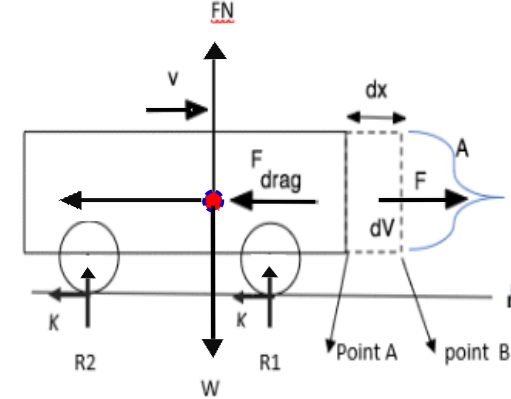
\includegraphics[width=0.7\textwidth]{cardynamics}
\caption{Forces of Vehicle Dynamics.}
\label{fig:cardynamics}
\end{figure}

This section describes how a vehicle reacts to a given force  input as reflected in figure  \cref{fig:cardynamics}. Assuming that the above vehicle image  \cref{fig:cardynamics}  is moving in a horizontal plane, the list of forces that will act on it and other relevant variables are listed below:
\begin{description}
  \item $[F]-Tractive force$; This is the force delivered by the car engine  to the wheel via the gear and the axil system.
  \item $[K]-Frictional force;$ This exist between the tire and the road surface. The wheels push backwards on the road surface and, in reaction, the road surface pushes back in a forward direction.
  \item $[FN]- Normal force$ ; It act perpendicular to the car position.
  \item[W]- Weight of the car
  \item[V]-Car velocity
  \item$ [C_{drag}] $- This is the parallel force acting in the same direction as the airflow.
  \item $[F_{drag}]-Drag Force $; This is the wind or air resistance force acting in the opposite direction of the motion.
  \item[A]- Defines the area of the vehicle which the drag force is acting upon
  \item[dx]- Distance covered by the vehicle from point A to point B
  \item[Red dot]- Centre of gravity of the vehicle
  \item[R1 and R2]- Reaction force on the tire from the ground
 \end{description}

\subsection{Frictional Force}
The frictional force exerted on the tire of a vehicle "Fr" is the product the coefficient of static friction $"\mu"$,  the mass "m" and the acceleration due to gravity "g" and it resist relative motion. The model of the frictional force is dependent on the following:
\begin{itemize}
    \item Reaction force; Exerted by the surface on the object (this is in accordance with the Newton's 3rd Law of motion), this force has an equal magnitude to the object weight and it act in upward direction \ref{eqn:reactionforce}.
    \begin{equation}
     \mbox{R} = W = m \cdot g
     \label{eqn:reactionforce}
    \end{equation}

\item Coefficient of Static Friction: This correspond to the roughness of the surface, usually this value lies between 0 and 1 and increases as the roughness of a surface increases, this is denoted by $\mu$.\\
\end{itemize}
Therefore we model the frictional force thus\ref{eqn:frictionalforc}:
\begin{equation}
 \mbox{Fr} = \mu \cdot m \cdot g % assuming a flat surface road path
 \label{eqn:frictionalforc}
\end{equation}


\subsection{Engine force}
A car engine delivers an amount of torque.  Torque is like a rotational equivalent of force. Torque is force times distance. The torque that an engine can deliver depends on the speed at which the engine is turning, expressed as rpm (revolutions per minute). The relationship between torque versus rpm is not a linear one but, is usually provided as a curve known as a torque curve.\\
However, the torque from the engine (i.e. at the crankshaft) is converted via the gear and differential before it's applied to the rear wheels. The gearing multiplies the torque from the engine by a factor depending on the gear ratios. Also, the torque on the rear axle can be converted to a force of the wheel on the road surface by dividing by the wheel radius. (Force is torque divided by distance).
We can drive the drive force from an equation to get from engine torque to drive force: the longitudinal force that the two rear wheels exert on the road surface.
\begin{equation}
  F_{drive} = u * T_{engine} * x_{g} * x_{d} * n / R_{w}
\end{equation}
  where
    u is a unit vector which reflects the car's orientation,
   $ T_{engine}$ is the torque of the engine at a given rpm,
   $ x_{g} $ is the gear ratio,
    $x_{d}$ is the differential ratio,
    n is transmission efficiency and
    $R_{w}$ is wheel radius.

Vehicle engine delivers an amount of torque, which  is the measurement of how quickly the vehicle will accelerate, which is determined by the speed of engine turning ($Torque = force \cdot distance$). Torque from the engine (i.e. at the crankshaft) is converted via the gear and differential before applying it to the rear wheels \ref{eqn:enginforce}\\
However, the engine torque acts on the vehicle wheel by dividing by the wheel radius.

\begin{equation}
 \mbox{engine torque} = throttle \; position \cdot max \; torque
 \label{eqn:enginforce}
\end{equation}

Torque is delivered to the drive wheels via the gearbox and it's results in the drive torque \ref{eqn:drivetorque}:

\begin{equation}
 \mbox{drive torque}  = engine \;torque \cdot gear \; ratio \cdot differential \; ratio \cdot transmission \; efficiency \
 \label{eqn:drivetorque}
\end{equation}

   \begin{equation}
    \mbox[{F_{traction}}  = {u \cdot \mbox Engine_{force}} ] % I recommend to put long strings in mbox
    \label{eqn:tractionforce} % not use equation* normally
   \end{equation}

   where u is a unit vector in the direction of the vehicle.\\

   The air resistance forces otherwise called the  drag equal to
   \begin{equation}
   \mbox[{F_{drag}} =  - C_{drag} \cdot v \cdot |v| ]
   \label {eqn:airresistance}
   \end{equation}% ALWAYS use \cdot
   where $C_{drag}$ is a constant, v is the velocity vector and $|v|$ is to the magnitude of vector v\\
There is the rolling resistance force which is caused by friction between the tire and road surface as the wheels roll along.

\begin{equation}
[F_{rr} = - C_{rr}  \dot v]
\label{rollingresistance}
\end{equation}
where $C_{rr}$ is a constant and v is the velocity vector\\

Therefore, the total longitudinal force equals the vector sum of these three forces \ref{eqn:longitudinalforce}.\\
\begin{equation}
\mbox [ {F_{long}} =   F_{traction} + F_{drag}  +  F_{rr}]
\label{eqn:longitudinalforce}
\end{equation}
It is observed that if driving in a straight-line, the drag and rolling resistance forces will be in the opposite direction from the traction force. Using the graph in \ref{fig:Velocitytimegraph} to illustrate the impact of velocity on a moving vehicle with respect to time.

\begin{figure}
    \centering
    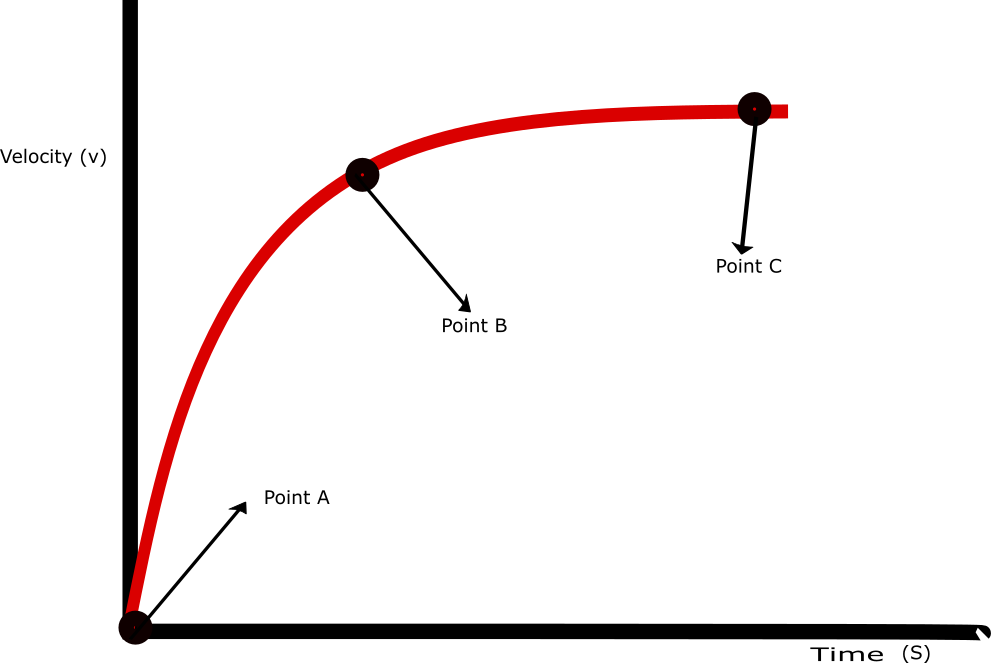
\includegraphics[width=0.7\textwidth]{text3864}
    \caption{Velocity time graph.}
    \label{fig:Velocitytimegraph}
\end{figure}

The graph in \ref{fig:Velocitytimegraph}  explains the impact of the forces acting on a moving car changes with change in car speed.\\
\begin{itemize}
    \item Point A:  Is the beginning of the car movement; the driving force “F” is greater than the air resistant “A”\\
    \item Point B; The velocity and, air resistance increases, while the resultant force decreases with lower acceleration rate.\\
    \item Point C; The driving force is balanced by the air resistance, the velocity stops increasing (this is called terminal velocity).
\end{itemize}

\newcommand{\esymbol}[1]{\textbf{\textit{#1}}}

\subsubsection{Gear Ratios}
According to {\url{http://www.davette.net/facts/c5specs/}}, below gear ratios apply to Corvette C5 hardtop

\begin{center}
\begin{tabular}{ |c|c|c| }
 \hline
 Gear No & Abbreviation  & Ratio \\
  \hline
 First gear &  g1  & 2.66 \\
  \hline
  Second gear &  g2  & 1.78 \\
  \hline
   Third gear &  g3  & 1.30 \\
  \hline
   Fourth gear &  g4  & 1.0 \\
  \hline
    Fifth gear &  g5  & 0.74 \\
  \hline
  Sixth (!) gear &  g6  & 0.50 \\
  \hline
  Reverse gear &  grR & 2.90 \\
  \hline
  Differential ratio & xd & 3.42\\
  \hline
\end{tabular}
\end{center}


The combination of gear and differential acts as a multiplier from the torque on the crankshaft to the torque on the rear wheels, also in low gears the gear ratio is high, so you get lots of torque but not so much speed. In high gears, you get more speed but less torque.

engine torque = throttle position * max torque

This torque is delivered to the drive wheels via the gearbox and results in what I'll call the drive torque:

    $ drive_torque = engine_torque * gear_ratio * differential_ratio * transmission_efficiency $

Or written more concisely as:

   $ Tdrive =  Tengine * xg * xd * n $
Because $F_{drive} = T_{drive} / Rw $ , this is the same as the equation for drive force we saw earlier. Meanwhile, the gearbox increases the torque, but reduces the rate of rotation, especially in low gears.


\section{Acceleration}
Acceleration which is the rate of change of velocity of an object with respect to time, according to Newtons law, an object's acceleration is the net result of all forces acting on it.
The SI unit for acceleration is metre per second squared $(m \cdot s^2)$. Accelerations is a  vector quantity which is added according to the parallelogram law. The net force vector acting on a body has the same direction as the vector of the body's acceleration, and its magnitude is proportional to the magnitude of the acceleration, with the object's mass (a scalar quantity) as proportionality constant.

For instance, when a stationary car (zero velocity, in an inertial frame of reference) travels in a straight-line at increasing speeds, it is accelerating in the direction of travel, when the car turns, an acceleration occurs toward the new direction. The forward acceleration of the car is called a linear (or tangential) acceleration. Passengers in the car experience a force pushing them back into their seat, but When changing direction (orthogonal to tangential) acceleration, the passengers experience a sideways force. If the speed of the car decreases, this is an acceleration in the opposite direction of the velocity of the vehicle, sometimes called deceleration or retrograde burning in spacecraft.[4] Passengers experience  deceleration as a force pushing them forwards. Both acceleration and deceleration are as a result of changes in velocity.Tangential, radial or deceleration force is being felt by passengers until their velocity (speed and direction) matches that of the uniformly moving car.
The average acceleration over a period is its change in velocity (Dv) divided by the duration of the period (Dt).  Mathematically, we have

Acceleration is the rate of change of velocity. It is the amount that velocity changes per unit time.

If an object accelerates from an initial velocity (u) up to a final velocity (v) then the average acceleration of an object can be calculated using the equation:
ACCELERATION = change in velocity/time: a = (v-u)/t


The acceleration \esymbol{"a"} of a vehicle is determined by the components of net force \esymbol{"F"} and the car's mass \esymbol {"M"}

\begin{eqnarray}\label{eq:2}
F = m \cdot a    \ (in \ Newtons) \
\end{eqnarray}
Therefore
\begin{eqnarray}
\esymbol[{a} = \left(\frac{F}{m}\right)  \  { \left( in \ \frac{meters}{ seconds^2}\right) }]
\end{eqnarray}

According to Euler method for numerical integration, the vehicle velocity (in meters per second) is determined by integrating the acceleration over time :
\begin{equation}
   v =  v + dt * v
\end{equation}

dt is the time increment  in seconds between call of the physics engine \\

Also, the vehicle position is the integral of velocity over time :
 \begin{equation}
   p = p + dt * v
 \end{equation}

 The above three forces can execute the following functions
 \begin{itemize}
     \item Simulate car acceleration objectively accurate
     \item They can be used to calculate the top speed of a car for a given engine power
     \item The velocity increase proportional to the resistance force increment while the net for decreases with decrease in acceleration.
     \item At the car top speed, the resistance force cancels the engine force.
 \end{itemize}

\begin{figure}
\centering
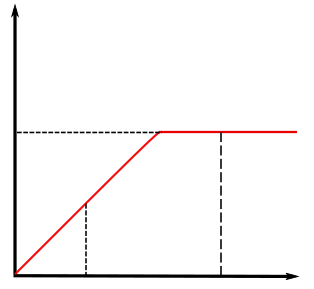
\includegraphics[width=15cm,height=10cm]{Velocitycumtimegraph}
\caption{Velocity-Time graph}
\label{fig:velocityforce}
\end{figure}
 From the figure \cref{fig:velocityforce} X-axis denotes car velocity while the y-axis is the force values. \\
 The rolling resistance (dotted line) is a linear function of velocity and the drag (thick curve) is a quadratic function of velocity while the traction force(red line) does not depend on the velocity of the car.\\
 It is observed that the value of the constants above should reflect the reality in car driving, so the speed of the car movement is highly dependents on the two constant $c_{drag}$ and $c_{rr}$, hence the need to assign a value that is reasonable to them. \\
 The air resistance is approximated as :
 \begin{equation}
   f_{drag} = 0,5 * c_d * A * rho * v ^ 2
 \end{equation}
where Cd = coefficient of friction whose values depends on car shape
    A is frontal area of car = 2.2m (20 square feet)
    rho is = density of air which is equal to 1.28km/m ( 0.0801) to
    v = speed of the car

 Therefore, $C_{drag}$  = $0.5 * 0.30 * 2.2 * 1.29 = 0.4257$

 Recall that $C_{rr}$ should be approximately 30 times $C_{drag}$.  This gives us
    $C_{rr} = 30 * 0.4257$
          $= 12.8$

\begin{eqnarray}
\textit [{a} = \textit{m} \cdot \textit{Dv} / {Dt}]
\end{eqnarray}

The acceleration \esymbol{a} of the vehicle is determined by the net force on the car and the car's mass \esymbol{m}:\\
\begin{eqnarray}
\textit{F} = \textit{m} \cdot \textit{a} \qquad [F] = (\frac{m}{ s^2})
\end{eqnarray}

Therefore,
\begin{eqnarray}
[Fr = \textit{uHf} \cdot \textit{g} \cdot \textit{m} / 2 ]
\end{eqnarray}

Assume friction of $ 0.5 $
\begin{eqnarray}
 F = m \cdot a \\ % solve for a
 a = uHf \cdot g / 2
\end{eqnarray}
The car's position can easily be update by
\begin{equation}
  p = dt \cdot v
\end{equation}



\section{Vehicle Deceleration (Braking force)}
Deceleration is the opposite of acceleration or otherwise called negative acceleration. In this situation, the traction force is replaced by a braking force which is oriented in the opposite direction. The deceleration force is due to the braking force generated between the tire and the road surface. This force is a product of the coefficient of friction $" \mu Hf"$ and the normal force 'Fn'\\
With reference to equation \ref{eq:2},
\begin{eqnarray}
%\mbox{F}  = m \cdot a  \\
\mbox{Fr}  = \mu Hf\cdot Fn = uHf\cdot g \cdot m \ (in \ Newtons) \\
\mbox{deceleration:} \  a = - uHf \cdot g  \  { \left( in \ \frac{meters}{ seconds^2}\right) }
\end{eqnarray}

When braking, the traction force is replaced by a braking force which is oriented in the opposite direction.
\mbox{distance to start breaking is:}
\begin{equation}
d = \frac{1}{2} \cdot  v^2/a
\end{equation}
The total longitudinal force which is then the vector sum of these three forces is equivalent to:
\begin{equation}
[F_{long} =   F_{braking} + F_{drag}   + F_{rr}]
\end{equation}

Therefore, breaking model;
\begin{equation}
\mbox{Fbraking} = -u \cdot Cbraking
\end{equation}

It is important to make sure that you stop applying the braking force as soon as the speed is reduced to zero otherwise the car will end up going in reverse.

\subsection{Vehicle deceleration:} Deceleration is the opposite of acceleration or otherwise called negative acceleration.\\
deceleration (straight)

\begin{eqnarray}
\mbox{F}  = m \cdot a
\mbox[{Fr}  = uHf\cdot Fn = uHf\cdot g \cdot m]  %(for all 4 tires, see acceleration)
\mbox[{deceleration:}  a = uHf \cdot g] % (it is negative acceleration)
\end{eqnarray}




\section{Force at a curve}

The centripetal force "Fpetal" is acting on the vehicle towards the centre direction of the curve at an intersection. This is the force that acts on a vehicle moving in a circular path
At this stage, keeps speed constant, assume no over-steering, "r" is the radius of the curve, the tangential velocity "v", the vehicle mas "m"
\begin{eqnarray}
\mbox{Fpedal} = m \cdot v^2/r  \ (in \ Newtons) \\
\mbox{To avoid slipping out of the curve,} \
\mbox{solve for} \; Fr >= FPedal  \ (in \ Newtons)\\
 v <= sqrt (uHf \cdot g \cdot). \ (in \ meter \ per \ second)
 \end{eqnarray}


At a curved road path, the centripetal force acts on the vehicle towards the centre direction of the curve. This force is directed toward the centre around which the car is moving, which makes the vehicle to move in a circular path. As indicated in \ref{fig:overshootingcar}, the speed  is kept constant, assumes over-steering, r is the radius of the curve.



As indicated in the figure below;
\begin{figure}[tbp]
  \centering
  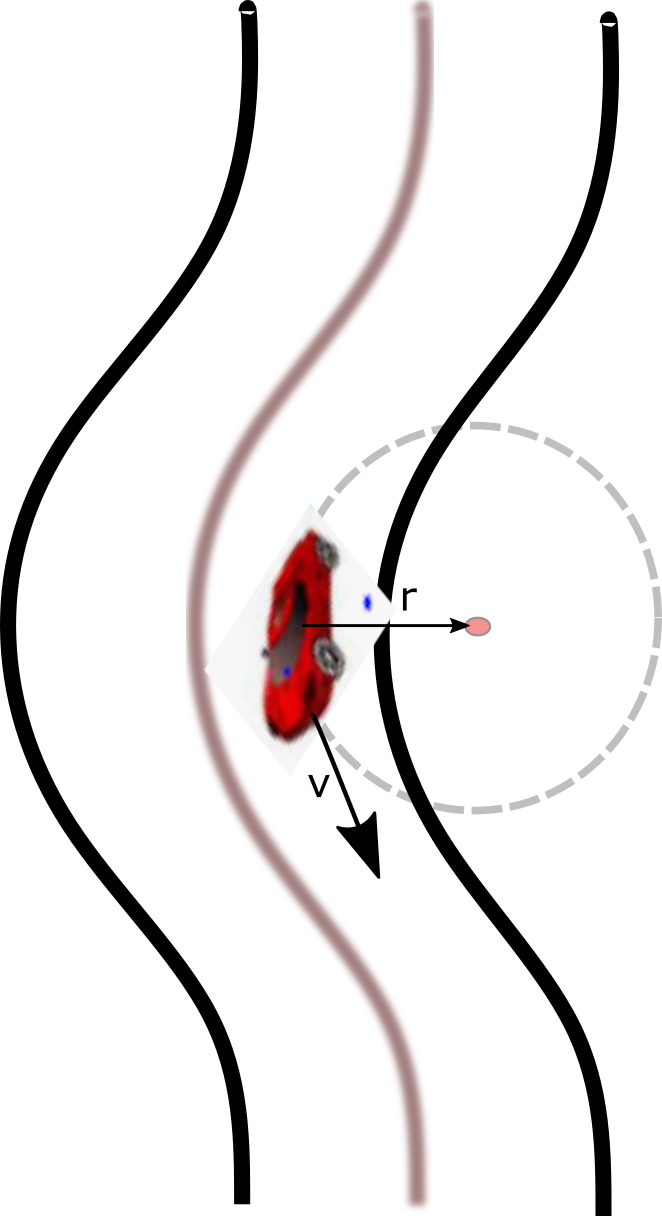
\includegraphics[width=0.4\textwidth]{text11376}
  \caption{Over-shooting vehicle in a curve}
  \label{fig:overshootingcar}
\end{figure}

\begin{figure}[htbp]
  \centering
  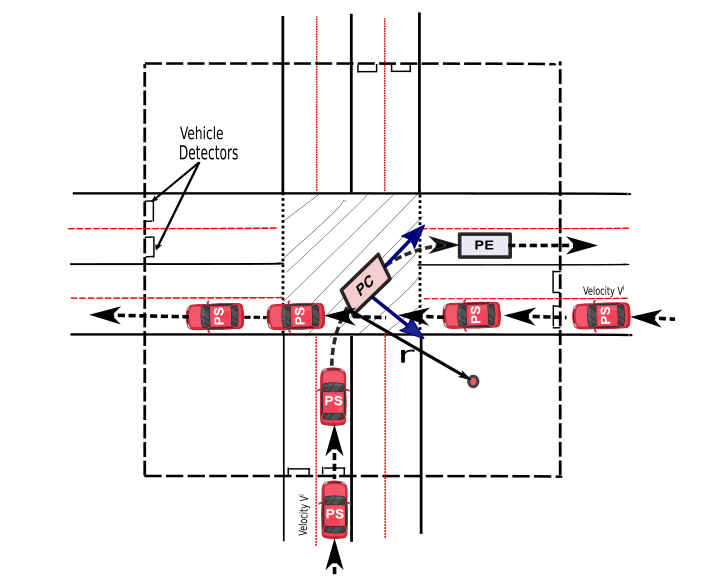
\includegraphics[width=1.0\textwidth]{CollisionVehicle.PNG}
  %\centering{\includegraphics[width=0.6,height=0.6,keepaspectratio]{Figure}}
  \caption{Cross Collision vehicles}
\end{figure}

At this stage, keep speed constant, assume now over-steering, r is the radius of the curve
\begin{eqnarray}
\mbox{FPedal} = m \cdot v^2/r
\mbox{Solve for} \; Fr >= FPedal  % (to avoid slip out of the curve)
 v <= sqrt (uHf \cdot g \cdot)
\end{eqnarray}


%\setcounter{Driving in a Curve }
\begin{figure}
\centering
  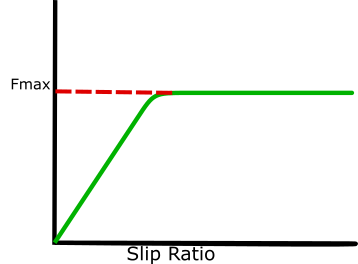
\includegraphics[width=0.5\textwidth]{text3784}
 \caption{Curved Movement}
  \label{fig:CurvedMovement}
\end{figure}

It is important to note that simulating the car to turn at low speed is different from turning at high speed; at low speeds (parking), the wheels pretty much roll in the direction they're pointed at. To simulate this, you need some geometry and some kinetics. You don't really need to consider forces and mass. In other words, it is a kinetics problem not a dynamics problem, at higher speeds, it becomes noticeable that the wheels can be heading in one direction while their movement is still in another direction. In other words, the wheels can sometimes have a velocity that is not aligned with the wheel orientation. This means there is a velocity component that is at a right angle to the wheel. This of course causes a lot of friction. After all a wheel is designed to roll in a direction and that without too much effort. Pushing a wheel sideways is very difficult and can generate a lot of frictional force. In high speed turns, wheels are being pushed sideways and we need to take these forces into account also\\
Considering a low speed cornering, we can assume that the wheels are moving in the direction they're pointing, which means that the wheels are rolling, but not slipping sideways.  If the front wheels are turned at an angle delta and the car is moving at a constant speed, then the car will describe a circular path.  We place our emphases on the steering angle of the front wheel at the inside of the curve and ignore the wheel at the other side.
\begin{figure}[htbp]
  \centering
  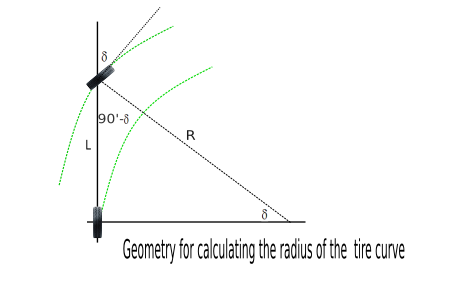
\includegraphics[width=0.9\textwidth]{radiusofacurve}
  \caption{Curved radius calculator}
  \label{fig:curvedradius}
\end{figure}

Using geometry, the radius of the circle could be determined as reflected on the below diagram \ref{fig:curvedradius}\\
where L = distance between front and rear axle\\
    R = radius of the circle the front wheel describes\\
    The angle at the rear wheel is 90 degree, at the front wheel is 90 degrees minus $\delta (90-\delta)$, which means that the angle at the centre is also delta(sum of angles in a straight-line = 180).\\
  Therefore,
  \begin{equation}
    sin (\delta) = L/R - R = L/sin(\delta)
  \end{equation}

Note that if the steering angle is zero, then the circle radius is infinite, i.e. we're driving in a straight-line. \\

The next step is to calculate the angular velocity  $\omega$, i.e. the rate at which the car turns. This is expressed in radiant per second. (A radian is a full circle divided by $ 2 \pi$)\\
 Therefore
\begin{equation}
  \omega = V/R
  \end{equation}
From the above two equations, we know how fast the car must turn for a given steering angle at a specified speed.\\
Note:\\
\begin{itemize}
\item The steering angle is determined from user input.
\item The car speed is determined as for the straight movement (vector2) always points in the car direction).
\item From this we calculate the circle radius and the angular velocity which is used to change the car orientation at a specific rate.
\end{itemize}

\subsubsection{High Speed Turning}
At high speeds, we can no longer assume that car wheels are moving in the direction they're pointing because of to the car body which has a certain mass and  takes time to react to steering forces. Just like linear velocity, this takes time to build up or slow down.  This is determined by angular acceleration which is in turn dependent on torque and inertia (which are the rotational equivalents of force and mass). However, thinking of a driver going under a curve, car may be pointing in one way but moving another way. The  angle between the car's orientation and the car's velocity vector is known as the sideslip angle (beta).\\
\begin{figure}[htbp]
  \centering
  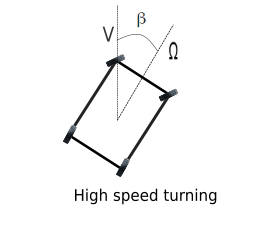
\includegraphics[width=0.9\textwidth]{speedturning}
  \caption{Slip angle (Angle between the car's orientation and car's velocity)}
\end{figure}
A scenario of high-speed cornering from the wheel's point of view, in this situation we need to calculate the sideways speed of the tires, because wheels rolls with relatively low resistance to motion in forward or rearward direction, but the perpendicular direction has great resistance to motion. Pushing a car sideways is very hard because you need to overcome the maximum static friction force to slip the wheel. In this situation, the tires develop lateral forces also known as the cornering force, which force depends on the slip angle "alpha" ( which exist between the tire's heading and its direction of travel). As the slip angle grows, so does the cornering force also but the cornering force per tire also depends on the weight on that tire. At low slip angles, the relationship between slip angle and cornering force is linear, in other words:\\

$F_{lateral} = Ca * alpha $\\

where the constant Ca  is known as the cornering stiffness.
Using the diagram bellow to explain this, the vector2 of the wheel has angle alpha relative to the direction in which the wheel can rolls. Vector2 consist of two component vectors:
\begin{itemize}
    \item The longitudinal vector whit magnitude $ cos(\alpha) * v $. Movement in this direction corresponds to the rolling motion of the wheel.
    \item The lateral vector with magnitude $ sin(\alpha) * v $ which causes a resistance force in the opposite direction of the cornering force.
\end{itemize}

\begin{figure}[htbp]
  \centering
  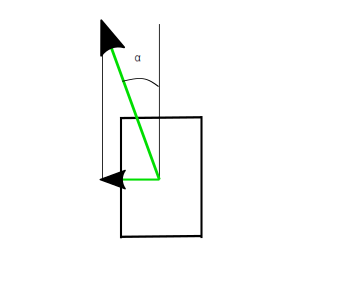
\includegraphics[width=0.9\textwidth]{wheelongilateral}
  \caption{Longitudinal and lateral velocity vectors of wheel}
\end{figure}

The slip angle is determined by  the sideslip angle of the car, the angular rotation of the car around the up axis (yaw rate) and, for the front wheels, the steering angle.\\
The sideslip angle $\beta$ is the difference between the car orientation and the direction of its movement, in other words the angle between the longitudinal axis and the actual direction of travel. So it's similar in concept to what the slip angle is for the tires. Because the car may be moving in a different direction than where it's pointing at, it experiences a sideways motion. This is equivalent to the perpendicular component of the velocity vector.

\begin{equation}
   [ \beta = arctan(v_{y}/v_{x})]
\end{equation}
But If the car is turning around the centre of geometry (CG) at a rate omega (in rad/s), it means that the front wheels are describing a circular path around CG at same rate. If the car turns full circle, the front wheel describes a circular path of distance $ 2.\pi.b $ around CG in $ 1/(2.\pi.\omega)$ seconds where b is the distance from the front axle to the CG. This means a lateral velocity of $ \omega * b $. For the rear wheels, this is $\-omega * c $. Note the sign reversal. To express this as an angle, take the arctangent of the lateral velocity divided by the longitudinal velocity (just like we did for beta).  For small angles we can approximate $ arctan(vy/vx) by vx/vy $.
\begin{figure}[htbp]
  \centering
  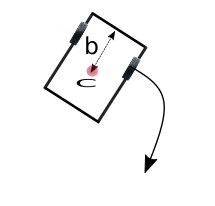
\includegraphics[width=0.9\textwidth]{circularpathfront}
  \caption{Circular path front wheel angle movement}
\end{figure}

The steering angle $ (\delta) $ is the angle that the front wheels make relative to the orientation of the car. There is no steering angle for the rear wheels, these are always in line with the car body orientation. If the car is reversing, the effect of the steering is also reversed.
\begin{figure}[htbp]
  \centering
  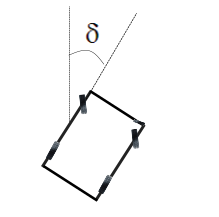
\includegraphics[width=0.9\textwidth]{Steeringangle}
  \caption{steering angle}
\end{figure}

The slip angles for the front and rear wheels are given by the following equations:

\begin{equation}
\alpha[_{front} = arctan[(v_{lat] + \omega *b)}\: / \: V_{long}]- \sigma. sin(v_{long})]
\end{equation}

\begin{equation}
 \alpha_{rear} = arctan[(v_{lat] - \omega * c)}\: / \; V_{long}]
\end{equation}

The lateral forces of the four tyres have two results: a net cornering force and a torque around the yaw axis.  The cornering force is the force on the CG at a right angle to the car orientation and serves as the centripetal force which is required to describe a circular path.  The contribution of the rear wheels to the cornering force is the same as the lateral force.  For the front wheels, multiply the lateral force with cos(delta) to allow for the steering angle.
\begin{equation}
  F_{cornering} = F_{lat, rear} + cos(delta) * F_{lat, front}
\end{equation}

As a point of interest, we can find the circle radius now that we know the centripetal force using the following equation
\begin{equation}
   F_{centripetal} = M v^2 / radius
\end{equation}

The lateral force also introduces a torque which causes the car body to turn.  After all, it would look very silly if the car is describing a circle but keeps pointing in the same direction.  The cornering force makes sure the CG describes a circle, but since it operates on a point mass it does nothing about the car orientation. That's what we need the torque around the yaw axis for \cite{van2003collision}.
Torque is force multiplied by the perpendicular distance between the point where the force is applied and the pivot point.
\begin{equation}
Rear wheels effect on the torque = -F_{at, rear} * c
\end{equation}

 While the front wheels it's .
\begin{equation}
 Front wheels effect on the torque = cos(delta) * F_{lat, front} * b
\end{equation}
 Note that the sign differs.
Applying torque on the car body introduces angular acceleration.  Just like Newton's second law F = M.a, there is a law for torque and angular acceleration:

Torque = Inertia * angular acceleration.

The inertia for a rigid body is a constant which depends on its mass and geometry (and the distribution of the mass within its geometry).

Distance is how far an object moves. It does not include an associated direction, so distance is a scalar quantity.
Speed is the rate of change of distance – it is the distance travelled per unit of time. Like distance, speed also does not have an associated direction, so, it is a scalar quantity.
SPEED = distance/time, while distance = average speed(velocity) * time



\subsection{Vehicle Slip and traction force}
This is the relative motion that exist between a tire and the road surface in a moving vehicle, the reaction to the wheel slipping  is what pushes the car forwards.  This frictional force produced is known as traction or longitudinal force.  This traction force depends on the amount of slip. Generating the wheel angular velocity from the car speed is only allowed if the wheel is rolling, which means that there is no lateral slip between the tire surface and the road.  This situation is true for the front wheels, but for drive wheels this is typically not true. After all, if a wheel is just rolling along it is not transferring energy to keep the car in motion. In a scenario where the car is cruising at constant speed, the rear wheels will be rotating slightly faster than the front wheels, because the front wheels are rolling and therefore have zero slip, the surface of the tire is slipping regarding the road surface. You can calculate their angular velocity by just dividing the car speed by "2 pi" times the wheel radius.   Hence the reaction force exerted due to the wheel slipping is what pushes the car forwards.  This friction force is known as traction or the longitudinal force which depends on the amount of slip (slip ratio)

For a simple simulation the longitudinal force can be approximated by a linear function:
\begin{equation}
\mbox[{F_{long}} = Ct \cdot slip \; ratio]
\end{equation}

where Ct is the traction constant, which is the slope of the slip ratio curve at the origin as indicated in \ref{fig:SlipAngle}\\
\begin{figure}[htbp]
  \centering
  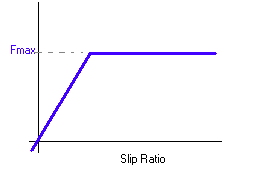
\includegraphics[width=0.9\textwidth]{Capture}
  \caption{Slip Angle}
  \label{fig:SlipAngle}
\end{figure}
In the alternative, for a more complex system we can calculate the slip ration denoted as $\sigma$ thus:\\

\begin{equation}
 [\sigma = (\omega_{w} . R_{w} - V_{lon})/ \mid V_{long} \mid]
 \label{eqn:carreversing}
\end{equation}

Where $\omega_{w}$ is the wheel angular velocity\\
$R_{w}$ is the wheel radius\\
$V_{long}$ is car speed ( the longitudinal velocity)

From equation \ref{eqn:carreversing}, works for a car deriving in reverse direction (note that cars have slip ratios of 0, -1 and + for a free rolling wheel, braking with cocked wheel, and accelerating forward respectively). Wheel grips best with a little bit of slip while decreasing the slip would give you more traction and better acceleration of a car. The force in the longitudinal direction is linear to the load or car weight.

\begin{equation}
 \mbox [F_{long} = F_{n, long} * F_{z} ]
\end{equation}

Where $F_{n, long}$ is the normalized longitudinal force, and $ F_{z} $ is the tire load


\begin{figure}[htbp]
  \centering
  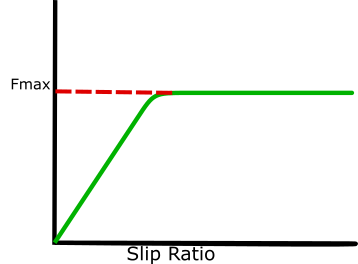
\includegraphics[width=0.9\textwidth]{text3784}
  \caption{Slip Angle}
\end{figure}

\subsection{Torque on the wheel} The wheel torque oppose the torque delivered by the engine (drive torque)\\
 traction torque = traction force  *  wheel radius.\\
 In a real-life scenario process of moving a car by the engine force, the engine torque is magnified by the gear and the differential ratio, and then provides the drive torque on the rear wheels.  The angular velocity of the wheel is high enough that it causes slip between the tire surface and the road, which can be expressed as a positive slip ratio. This results in a reactive friction force, known as the traction force, which is what pushed the car forward.  In this case the net torque is still positive and will result in an acceleration of the rear wheel rotation rate. This will increase the rpm and increase the slip ratio.

 \begin{figure}[htbp]
  \centering
  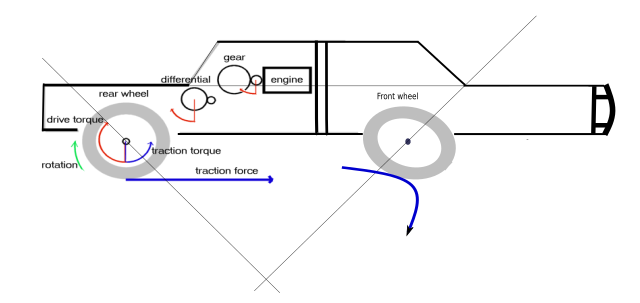
\includegraphics[width=0.9\textwidth]{enginegearwheelforce}
  \caption{Engine, gear, differential and wheel force impact}
  \label{fig:enginegearwheelforce}
\end{figure}



 From the diagram \ref{fig:enginegearwheelforce}, the total torque = drive torque + traction torques from both wheels + brake torque.\\ This torque will cause an angular acceleration of the drive wheels.\\
 The angular acceleration = total torque / rear wheel inertia.\\
 A positive angular acceleration will increase the angular velocity of the rear wheels over time. As for the car velocity which depends on the linear acceleration, we simulate this by doing one step of numerical integration each time we go through the physics calculation:
\begin{equation}
rear wheel angular velocity += rear wheel angular acceleration * time step
\end{equation}


where time step is the amount of simulated time between two calls of this function.  This way we can determine how fast the drive wheels are turning and therefore we can calculate the engine's rpm.

\subsection{Gears and Wheel Torque}
The ratio between two gears, is the ratio of the gear
diameters. Car transmission will typically have between three (for automatic drive system) and six (for manual drive system) forward gears and one reverse gear. The wheel toque can
be obtained using the following equation.
\begin{equation}
 Tw = Te  \cdot gk  \cdot G
\end{equation}
(Where Te is the engine torque, gk is the gear ratio of whatever gear the vehicle is
in and G is the final drive ratio).\\
The relationship between the engine turnover rate and the wheel angular
velocity is as follows.

\begin{equation}
w = 2\Pi \omega e / (60 \cdot gk \cdot G) % (assuming that the tires roll on the ground without slipping)
\end{equation}


However, with these forces, we can simulate car acceleration accurately.
Car velocity increases with an increase in resistance forces, therefore when the car reaches its top speed, the resistance force and the engine force cancel each other.\



\chapter{Designing the Advanced Hybrid Intersection Management Technique}

\section{Methodology}

How has this been developed?

\section{Algorithm}

\section{Simulation for Traffic in Intersections}
Autonomous Driven Vehicle and Human Driven Vehicle Control Model Design (AVHVCONTROL)

\subsection{Simulator Architectural Model}
This covers the design and implementation  of the high-level structure of the software. It involves the assembling the architectural elements in some well-chosen forms to satisfy the major functionality and performance requirements of the system, it also takes care of reliability, scalability, portability and availability. According to  Perry and Wolfe in \cite{kruchten2005architectural}:\\ Software architecture = {Elements, Forms, Rationale/Constraints}.\\
\begin{figure}[htbp]
  \centering
  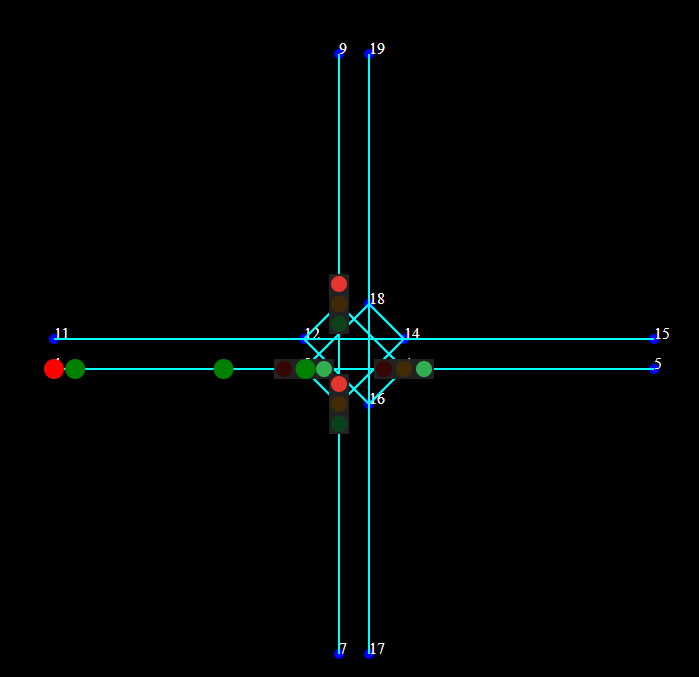
\includegraphics[width=0.9\textwidth]{crossjunctionsnap}
  \caption{Cross Road Intersection layout}
  \label{fig:componentsdiagram1}
\end{figure}
However, \cref{fig:componentsdiagram} addresses the architecture of this model, there is  concentrated on abstraction, decomposition, composition and applied the following majors views:
\begin{itemize}
    \item The logical view: This is the object model involving the functionality that the system provides to end-users
    \item View process: This captures the understanding that the model can be viewed as a "process" that has inputs, steps, and output(s) and that interfaces with other processes within the traffic network system.
    \item Physical view: This describes the mapping(s) of the software into the hardware system from the viewpoint of different stakeholders, such as end-users, developers, system engineer, and project managers.
    \item Development view: This describes the static organization of the software in its development
environment
\end{itemize}
In describing a model architecture—the decisions made—can be organized around these four views as listed above, with demonstrated scenarios or situations which integrates the functionality of each unit. \cref{fig:componentsdiagram} below demonstrates the different view in a software model architecture:

To analyse such mix or hybrid traffic scenario with reference to figure \ref{fig:tilesslot} , we  model HVs with navigation freedom and a worst-case scenario using a traffic light systems while the autonomous vehicle which can obey a stringent rule is centrally controlled using an intersection control unit with a strict respond to instruction at real time. In the design,  it is  important to consider the parameters that define the operation of each category of the vehicle without much deviation from the existing traffic infrastructure.\\
However, the differences between  HVs and AVs can be summarized under the following four heading:
\begin{itemize}
\item \textbf{Communication}: Autonomous vehicles are associated with a two-way communication system while human drivers are one way
    \item \textbf{Control Efficiency}: Autonomous observe a set of predefined rules, while human-driven vehicles have freedom. \cite{liu2018safe}.
    \item \textbf{Complexity in the set of rules}: Autonomous vehicles are protocol-based design(movement), while human nature control in HVs.
    \item \textbf{Response Time}:AVs response to instructions (emergency situations or braking) are automatic while HVs response time is 2.3 seconds\cite{mcgehee2000driver}.This delay can be dangerous in an emergency.
\end{itemize}

\subsection{Types of cars and its attributes}


\begin{center}
\begin{tabular}{ |c|c|c|c| }
 \hline
 type & properties1  & properties2 & properties2 \\
  \hline
 Human Driven cars & Non precision driving & Assumes aggressive driving & Uses driver to traffic light communications \\
  \hline
 Autonomous cars & Precision Driving & Defensive Driving & Uses V-v and V-I communication \\
 \hline
\end{tabular}
\end{center}


\subsection{Straight-line movement} First Scenario
Considering a car driving in a straight-line direction, the forces as listed below are at play:
\begin{itemize}
    \item Traction force: This is the force powered by the engine force transmitted to the car rear wheels. The engine when powered turns the axial through the gear system to the wheels (applies a torque on the wheel), the wheels push backwards on the road surface and, in reaction the road surface pushes back in a forward direction. The magnitude of this force is equivalent to the engine force. \\

    \begin{equation}
     \mbox [{F_{traction}} = { mu * engineforce }]
    \end{equation}

  Where mu is the coefficient of static friction and engineforce mass * acceleration due to gravity. In a scenario where this force is the only force acting on a vehicle, the vehicle will accelerate to infinity  but it is not the case in real-life situation because of drag.\\
  Drag force: This is the air resistance force which act in the opposite direction to the car movement, this force is proportional to the square of the car velocity.\\

     \begin{equation}
     \mbox[{F_{drag}} = { - C_{drag} * V * speed }]
    \end{equation}

  Where $C_{drag}$ is the drag coefficient (constant) and V is the velocity.\\
  However, speed is a scalar which is the magnitude of the velocity vector, hence we have :
     \begin{equation}
     speed = {(v.x * v.x + v.y * v.y)^ 1/2}
     f_{drag}.x  = {- C_{drag} * V.x * speed }
     f_{drag}.y = {- C_{drag} * V.y * speed}
    \end{equation}

  \item Rolling resistance force: This is a due to the friction between the car tires and the road surface :
  \begin{equation}
   F_{rr} = - C_{rr} * v
  \end{equation}
  where $C_{rr}$ is a constant while v is a velocity vector2
   \end{itemize}
    However, for a vehicle moving at a low speed, the rolling resistant is the main resistive force while the drag force acts  to resist the movement at high speed. therefore the total longitudinal force is the vector sum of the there three forces above
    \begin{equation}
   f_{long} = f_{traction} + f_{drag} + f_{rr}
  \end{equation}

Note
\begin{itemize}
    \item 1: For a vehicle moving in a straight-line direction, the rolling resistance force is in the opposite direction from the traction force which means that the magnitude of the resistance force is subtracted from the traction.
    \item 2. A car cruising at a constant speed, the above two forces are equal or in equilibrium ($f_{long} $ = 0)
\end{itemize}



\subsection{Car Weight impact}
The car weight has an effect on car motion when accelerating or braking with respect to the car tires. When braking hard on a high speed, the car will nosedive while during accelerating, the car leans back.  This is because just like the driver is pushed back in his seat when the pedal hits the metal, so is the car's centre of mass. The effect of this is that the weight on the rear wheels increases during acceleration and the front wheels conversely have less weight to bear. The effect of this is important because of the car weight distribution impact the maximum traction force at each of the four wheel due to friction limits and making the simulation real-life like.

\begin{equation}
  F_{max} = mu * W
\end{equation}
Where mu is the friction coefficient while W is the weight of the car.\\
However, for stationary vehicle, the weight of a car weight is distributed over the front and rear wheels according to the distance of the rear and front axle to wheels with \ref{eqn:carweight}
\begin{equation}
  w= M * g
  \label{eqn:carweight}
\end{equation}

Where
\begin{equation}
  W_{f} = (c/L)* W
\end{equation}
$W_{f}$ is the front wheel weight, c is the distance from the centre of gravity to rear axle and L is the wheel base

\begin{equation}
   W_{r} = (b/L)* W
\end{equation}
where  $W_{r}$ is the rear wheel weight, b is the distance from the centre of gravity to front axle and L is the wheel base
For instance, in a situation where the car is accelerating or decelerating at rate a, the weight on front ($W_{f}$) and rear axle ($W_{r}$) can be calculated as follows:
   \begin{equation}
    W_{f} = (c/L)*W - (h/L)*M*a
    W_{r} = (b/L)*W + (h/L)*M*a
   \end{equation}
  Where h is the height of the CG, M is the car's mass and a is the acceleration (negative in case of deceleration)




\subsubsection{How do we get the RPM}

So we need the rpm to calculate the engine's max torque and from there the engine's actual applied torque. In other words, now we need to know has fast the engine's crankshaft is turning.

The way I do it is to calculate this back from the drive wheel rotation speed.  After all, if the engine's not declutched, the crankshaft and the drive wheels are physically connected through a set of gears. If we know the rpm, we can calculate the rotation speed of the drive wheels, and vice versa!

rpm = wheel rotation rate * gear ratio * differential ratio * 60 / 2 pi. (The 60 / 2 pi is a conversion factor to get from rad/s to revolutions per minute.  There are 60 seconds in a minute and 2 pi radians per revolution )



\section{Vehicle Physics Model}
In vehicle physics, it is very important to separate the longitudinal( force which operates in the car direction or in its direct opposite direction)and that of the force acting laterally.\\
the above forces constitute of the following
\begin{itemize}
    \item Car wheel force
    \item Breaking force
    \item Rolling resistance force
    \ Drag or air resistance force
\end{itemize}
The above four forces are responsible for the controlling of car speed, acceleration and deceleration forces
For the purpose of this model, we made the following assumptions:
\begin{itemize}
    \item Notation is based on 2-dimensional vectors (vector2)
    \item the rear wheel is responsible for providing all the drive
    \item
\end{itemize}



\section{Experimental Results}

\subsection{ Simulator Model}
\subsection {Intersection routing using SVG}
 \begin{itemize}
     \item Development of intersection + cars moving
     \item Cars to become a self-aware “Agent”
     \item assign goals to cars
     \item Path-planning model
     \item Time step where they make decisions to prevents collisions and stuff
 \end{itemize}


\textbf{Pricing of road-spacetime and slot reservations for vehicles} is proposed. Airplanes use landing slots pricing to avoid conflict, what if AVs and HVs did the same thing in addition to platooning \cite{gong2018cooperative, calvert2011modelling, khondaker2015variable, swaroop1994comparision, chan2012cooperative}. Figures   \ref{fig:tilesslot} represent the intersection area for the scheme and vehicle reservation tiles respectively


\section{Testing Code}
We applied refactoring method which is the process of extracting code and putting it into a different form, without modifying its current behaviour. This is an excellent method of improving the code design of a program; and because any change could modify the behaviour of the simulator , it is safest to do when unit tests are in place. This module contains the core framework classes that form the basis of
specific test cases and suites (TestCase, TestSuite etc.), and a text-based utility class for running the tests and reporting the results



\section{Statistics}

\subsection{Vehicle Arrival Model}
Traditionally, Poisson distribution is used to model the random process, the number of vehicles arriving a given time period. We are going to apply discrete even simulation to handle the vehicle arrival model, the methodologies to generate random vehicle arrivals using random number of vehicles in each duration. Then we will elaborate various ways of evaluating the performance of a distribution.

Let t1, t2, t3 and t4 be four equal time intervals, then the number of vehicles arrived in each of these intervals is an integer value. For example, in if we have 3, 2, 3 and 1 vehicles arrived in time interval t1, t2, t3 and t4 respectively. Any discrete distribution that best
fit the observed number of vehicle arrival in each time interval can be used. Also, any continuous distribution that best fit the inter-arrival time can be used in the model, hence our process can be modelled first by modelling the number of vehicles that arrive at a given duration of time. Poisson distribution is idle to describe such a random process of car arrival.\\
The Poisson distribution is a discrete function, meaning that the event can only be measured as occurring or not as occurring, meaning the variable can only be measured in whole numbers.

The probability density function  p(x)
\begin{equation}
    p(x) = (\mu^x . e^{-\mu})\div x!
\end{equation}
where x = no of events will occur in time interval
    mu = expected rate of occurrence of that event
However, Since the events are discrete, the probability that certain number of vehicles (n) arriving in an interval can be computed as:
\begin{equation}
    p(x\leq n) = \sum_{i=0}^{n} p(i), i\in I
    \end{equation}

Similarly, the probability that the number of vehicles arriving in the interval is exactly in a range (between a and b, both inclusive and a < b) is given as:
\begin{equation}
    p(a\leq x \leq b) = \sum_{i=a}^{i} p(i), i\in I
    \end{equation}


    A simulation example: The hourly flow rate in a road section is 120 vph. Use Poisson distribution to model this vehicle
arrival
Solution: The flow rate is given as $(\mu) = 120 vph = 120/60 = 2$ vehicle per minute. Hence, the probability of zero vehicles arriving in one-minute p(0) can be computed as follows:
Therefore
\begin{equation}
   p(0) = (\mu^x . e^{-\mu}) \div x!  = (2^0 . e^-2)\div 0!   = 0.135
\end{equation}

%\section{Early Results}

%A first test was conducted to showcase the use of the simulator and to demonstrate the extraction of metrics from it.
%In this primitive scenario, cars were randomly moving within the intersection. Figure \ref{fig:graphcrashes} shows a plot of the number of vehicle %collisions against the number of vehicles in an intersection, at each time interval the number of cars in the intersection was taken in relation to %the number of collisions. From here we will categorize the cars based on HV and AV, add a behavioural feature like - obstacle maneuvering  and other %feature, and review its safety and efficiency.

 %\begin{figure}
%\centering
%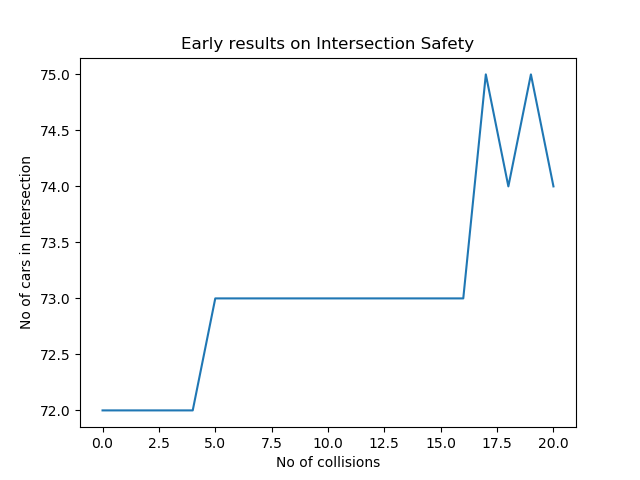
\includegraphics[width=8cm]{graph}
%\caption{Graph of no of cars versus no of crashes}
%\label{fig:graphcrashes}
%end{figure}


%\section{Summary}

%\jk{I would scratch that section}

%In summary, I have gathered, reviewed related work and constructed a classification matrix of both human driven and autonomous cars traffic management methods and started coding of a simulation model of car physical processes relevant in car movements dynamics.  In addition, I made a successful presentation at the opensource AI workshop and currently working towards a conference paper which the team of my supervisors plans to submit within the summer months.




%\section{physics Background }
%\centering
%\includegraphics{CarCurve1}
%\caption{\label{Figure:cardynamics} Direction of Centripetal Force}
%\end{figure}

%\section {Ethical issues associated with the integration of HV and AV}
the ethical challenges associated with AVs are summarized as shown below:
\begin{itemize}
  \item \textbf{Privacy Issues}: Running on sophisticated and advanced onboard computing systems, its communication standards are open for hacking \cite{amoozadeh2015security, collingwood2017privacy}
  \item \textbf{Morality issues} - the dilemma of taking a decision, for example Self trolley problem \cite{nyholm2016ethics, di2013self}
  \item \textbf{Safety Issues} ISO 26262 specify the
safety standard for road vehicles, what of AVs? google car test 1milion Kilometre, is this ok? \cite{koopman2017autonomous, kafka2012automotive,koopman2016challenges, birch2013safety}
  \item \textbf{Trust}- How trustworthy are the data source for navigation and route calculation are? \cite{yan2016can}
  \item \textbf{Transparency}- Transparency is a prerequisite for ethical engagement in AVs, while respecting copyright, corporate secrets, security
  \item \textbf{ Reliability}- What if there is no network of the sensor(s) fail? Possibility for having a threshold to determine car reliability
  \item \textbf{ Responsibility and Accountability}- in case of accident or incident, how does one determine responsibility \cite{lin2019autonomous,abduljabbar2019applications}
  \item \textbf{ Quality Assurance Process}- What is the overall quality and lifetime of components, quality control measures for transparent software engineering process
  \end{itemize}

\section {Some Open Source and Interface for AVs}

\jk{This geos to related work / background}

There is some open source interface platform for autonomous vehicle development, they include:
\begin{itemize}
\item Apollo - simulator engine
\item Autoware - open city driving in 3D maps
\item EB robinos and EB robinos Predictor  Elektrobit - combine software's together
\item NVIDIA® DriveWorks - Software kits -goes from detection to localization to planning to visualization.
\item OpenPilot - controls brake and steering system
\end{itemize}




\section{Software Testing}

In the course of testing this model, I applied the technique of 'unittest' for unit testing framework. This supports test automation, sharing of setup and shutdown code for tests, aggregation of tests into collections, and independence of the tests from the reporting framework which helped us to test the functionality of the individual parameters used in the model.

\section{ Tesla Cars}
Tesla, Inc. is a company based in Palo Alto, California which makes electric cars. ... It started selling its first car, the Roadster in 2008. The Tesla name originally comes from Nikola Tesla.
Things made: Electric vehicles; Tesla Energy

\bibliographystyle{plain}
\bibliography{Ref.bib}

\end{document}
